\documentclass[english,compress]{beamer}
\usepackage{kloeckislides}
\nonstopmode

\usepackage[normalem]{ulem}
\usepackage{pifont}
\usepackage{ifthen}

\setbeamercolor{section in head/foot}{use=structure,bg=structure.fg!25!bg}
\defbeamertemplate*{footline}{split theme}
{%
  \leavevmode%
  \begin{beamercolorbox}[wd=.5\paperwidth,ht=2.5ex,dp=1.125ex]{section in head/foot}%
    \insertsectionnavigationhorizontal{\paperwidth}{\hskip0pt plus1filll}{}%
  \end{beamercolorbox}%
  %\begin{beamercolorbox}[wd=.5\paperwidth,ht=2.5ex,dp=1.125ex]{subsection in head/foot}%
    %\insertsubsectionnavigationhorizontal{.5\paperwidth}{}{\hskip0pt plus1filll}%
  %\end{beamercolorbox}%
}


%\useoutertheme[subsection=false]{miniframes}

\setbeamertemplate{frametitle}[default][center]

\AtBeginDocument{%
  {
    \usebeamercolor{section in head/foot}
  }
  
  \pgfdeclareverticalshading{beamer@headfade}{\paperwidth}
  {%
    color(0cm)=(bg);
    color(1.25cm)=(section in head/foot.bg)%
  }

  \setbeamercolor{section in head/foot}{bg=}
}

\addtoheadtemplate{\pgfuseshading{beamer@headfade}\vskip-1.25cm}{}

\beamertemplatedotitem

\setbeamercolor{section in head/foot}{parent=palette quaternary}
\setbeamercolor{subsection in head/foot}{parent=palette primary}

\setbeamercolor{author in head/foot}{parent=section in head/foot}
\setbeamercolor{title in head/foot}{parent=subsection in head/foot}



\AtBeginSection[] {
  \begin{frame}<beamer>
  \frametitle{Outline}
  \tableofcontents[sectionstyle=show/shaded,subsectionstyle=show/show/hide]
\end{frame}
}
\AtBeginSubsection[] {
  \begin{frame}<beamer>
  \frametitle{Outline}
  \tableofcontents[sectionstyle=show/shaded,subsectionstyle=show/shaded/hide]
\end{frame}
}

\newcommand{\technicality}[2]{%
  {\strut #1\\
    \begin{beamercolorbox}[sep=1mm]{block body}
      #2
    \end{beamercolorbox}
  }%
}

\lstset{
  language=C++,
  rangebeginprefix=//\ ,
  rangeendprefix=//\ ,
}

\def\weblink#1#2{\href{#1}{\color{blue}\underline{#2}}}

\definecolor{fetch}{RGB}{227,110,35}
\definecolor{alu}{RGB}{255,188,24}
\definecolor{context}{RGB}{132,146,175}

\usepackage{keystroke}

\setbeamertemplate{navigation symbols}{}

\def\hilite<#1>#2{\alt<#1>{\colorbox{blue!30}{#2}}{\colorbox{white}{#2}}%
}

\lstset{
  language=C++,
  rangebeginprefix=/*\ ,
  rangeendprefix=/*\ ,
}

\begin{document}
% {{{ front matter

\title{High-Performance Scientific Computing\\Lecture 7: MPI Collectives, Intro to Performance}

\date{MATH-GA 2011 / CSCI-GA 2945 $\cdot$ October 17, 2012}

\frame{\titlepage}

\begin{frame}{Today}
  \tableofcontents[hideallsubsections]
\end{frame}
% }}}
% -----------------------------------------------------------------------------
\begin{frame}{Bits and pieces}
  \begin{itemize}
    \item HW3: reports out
    \item HW5: due today
    \item HW6: out tomorrow
    \item Project Pitches
  \end{itemize}
\end{frame}
% -----------------------------------------------------------------------------
\section[Valgrind]{Tool of the day: Valgrind}
% -----------------------------------------------------------------------------
\begin{frame}{Question}
  \textbf{Problem:} Debugging only deals with problems when they cause
  observable wrong behavior (e.g. a crash).

  \bigskip
  Doesn't find \emph{latent} problems.

  \bigskip
  \textbf{Suggested solution:} \emph{Monitor} program behavior
  (precisely) while it's executing. Possible?
\end{frame}
% -----------------------------------------------------------------------------
\begin{frame}{What is Instrumentation?}
  \begin{columns}
  \column{0.6\textwidth}
    What is Instrumentation?\\
    \hfill A.k.a. how does
    \weblink{https://secure.wikimedia.org/wikipedia/en/wiki/Valgrind}{Valgrind} work?

    \begin{center}
    \begin{tikzpicture}
    [every node/.style={draw,thick,fill=green!30,on chain,join,
    minimum height=4ex},
    every join/.style={thick,->},
    chain default direction=going below,
    node distance=3mm,
    start chain
    ]
    \node {x86(-64) Binary};
    \node {IR (SSA)};
    \node {Tool};
    \node {x86(-64) Binary};
    \end{tikzpicture}
    \end{center}

    \vspace{-0.7cm}
    Tools:
    \begin{itemize}
      \item Memcheck (find pointer bugs)
      \item Massif (find memory allocations)
      \item Cachegrind/Callgrind (find cache misbehavior)
      \item Helgrind/DRD (find data races)
    \end{itemize}

  \column{0.4\textwidth}
    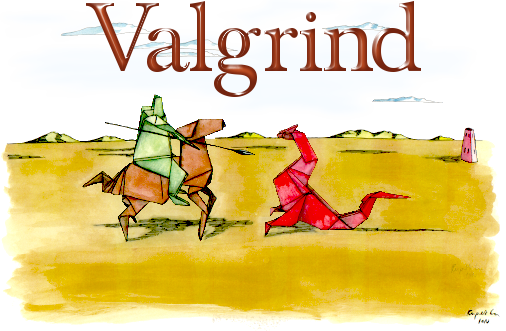
\includegraphics[width=\textwidth]{valgrind.png}
  \end{columns}
\end{frame}
\addimgcredit{Valgrind logo: Julian Seward}
% -----------------------------------------------------------------------------
\begin{frame}{Valgrind}
  \begin{center}
  \Huge Valgrind demo time
  \end{center}
\end{frame}
% -----------------------------------------------------------------------------
\section{MPI}
% -----------------------------------------------------------------------------
\subsection{Point-to-Point, Part II}
% -----------------------------------------------------------------------------
% {{{
\begin{frame}{MPI}
  \begin{center}
  \Huge Ordering demo recap
  \end{center}
\end{frame}
% -----------------------------------------------------------------------------
\begin{frame}{MPI: Ordering}
  \uncover<+->{}
  \textbf{MPI 3.0, Section 3.5:}
  \begin{quote}
    \upshape
    \textbf{Order} Messages are \hilite<+->{non-overtaking}: If a
    sender sends two messages in succession to the same destination,
    and both match the same receive, then this operation cannot
    receive the second message if the first one is still pending.

    \bigskip
    If a receiver posts two receives in succession,
    and both match the same message, then the second receive operation
    cannot be satisfied
    by this message, if the first one is still pending.
  \end{quote}
\end{frame}
% -----------------------------------------------------------------------------
\begin{frame}[fragile]{MPI: More on Ordering}
  Possible problem?
  \begin{lstlisting}
    if (rank == 0)
    {
      MPI_Bsend(buf1, count, MPI_DOUBLE, 1, tag1, comm)
      MPI_Ssend(buf2, count, MPI_DOUBLE, 1, tag2, comm)
    }
    else if (rank == 1) then
    {
      MPI_Recv(buf1, count, MPI_DOUBLE, 0, tag2, comm, status)
      MPI_Recv(buf2, count, MPI_DOUBLE, 0, tag1, comm, status)
    }
  \end{lstlisting}
\end{frame}
% -----------------------------------------------------------------------------
\begin{frame}{MPI: Progress}
  \textbf{MPI 3.0, Section 3.5:}

  \begin{quote}
    \upshape
    \textbf{Progress} If a pair of matching send and receives have
    been initiated on two processes, then at least one of these two
    operations will complete, independently of other actions in the
    system:

    \begin{itemize}
      \item the send operation will complete, unless the receive is
        satisfied by another message, and completes;
      \item the receive operation will complete, unless the
        message sent is consumed by another matching receive that
        was posted at the same destination process.
    \end{itemize}
  \end{quote}
\end{frame}
% -----------------------------------------------------------------------------
\begin{frame}{MPI}
  \begin{center}
  \Huge Non-overtaking demo time
  \end{center}
\end{frame}
% }}}
% -----------------------------------------------------------------------------
\subsection{Collectives}
% -----------------------------------------------------------------------------
% {{{
\def\collectivenodesmem#1#2{
  \foreach\rank in {0,1,2,3}
  {
    \foreach\memloc in {0,1,2,3}
    {
      \coordinate (#1-rank\rank-\memloc) at (\memloc,-\rank*1.25) ;
      \ifthenelse{\equal{#2}{1}}{
        \draw (#1-rank\rank-\memloc) ++(-0.5,-0.5) rectangle ++(1,1);
      }{}
    }
    \draw [ultra thick] (#1-rank\rank-0) ++(-0.5,-0.5) rectangle ++(4,1);
  }
  \coordinate (#1-tail) at ($ 0.5*(#1-rank2-3)+0.5*(#1-rank1-3) + (1,0) $);
  \coordinate (#1-head) at ($ 0.5*(#1-rank2-0)+0.5*(#1-rank1-0) - (1,0) $);
}
\def\collsetup#1{
  \collectivenodesmem{before}{#1}
  \begin{scope}[xshift=7.5cm]
    \collectivenodesmem{after}{#1}
  \end{scope}
  \draw [->] (before-head) ++(0.25,2) -- ++(0,-4)
  node [anchor=south,pos=0.5,rotate=90] {Ranks (Processors)};
  \draw [->] (before-rank0-0) ++(0,0.75) -- ++(3,0)
  node [anchor=south,pos=0.5] {Memory};
}
% -----------------------------------------------------------------------------
\begin{frame}{Broadcast}
  \begin{center}
    \begin{tikzpicture}[scale=0.85]

      \collsetup1
      \uncover<+->{}

      \node at (before-rank2-0) {17};

      \uncover<+->{
        \draw [thick,->] (before-tail) -- (after-head)
          node [above=2mm,pos=0.5,font=\ttfamily] {MPI\_Bcast} ;
      }
      \uncover<+->{
        \foreach\rank in {0,1,2,3}
          \node at (after-rank\rank-0) {17};
      }
    \end{tikzpicture}
  \end{center}
  \creditto{from Marsha Berger/David Bindel/Bill Gropp}
\end{frame}
% -----------------------------------------------------------------------------
\begin{frame}{MPI}
  \begin{center}
  \Huge Collectives demo time
  \end{center}
\end{frame}
% -----------------------------------------------------------------------------
\begin{frame}{Scatter}
  \begin{center}
    \begin{tikzpicture}[scale=0.85]

      \collsetup1
      \uncover<+->{}

      \foreach\i in {0,1,2,3}
        \node at (before-rank0-\i) {\pgfmathtruncatemacro{\res}{\i*2+5}\res};

      \uncover<+->{
        \draw [thick,->] (before-tail) -- (after-head)
          node [above=2mm,pos=0.5,font=\ttfamily] {MPI\_Scatter} ;
      }
      \uncover<+->{
      \foreach\i in {0,1,2,3}
        \node at (after-rank\i-0) {\pgfmathtruncatemacro{\res}{\i*2+5}\res};
      }
    \end{tikzpicture}
  \end{center}
  \creditto{from Marsha Berger/David Bindel/Bill Gropp}
\end{frame}
% -----------------------------------------------------------------------------
\begin{frame}{Gather}
  \begin{center}
    \begin{tikzpicture}[scale=0.85]

      \collsetup1
      \uncover<+->{}

      \foreach\i in {0,1,2,3}
        \node at (before-rank\i-0) {\pgfmathtruncatemacro{\res}{\i*2+5}\res};

      \uncover<+->{
        \draw [thick,->] (before-tail) -- (after-head)
          node [above=2mm,pos=0.5,font=\ttfamily] {MPI\_Gather} ;
      }
      \uncover<+->{
      \foreach\i in {0,1,2,3}
        \node at (after-rank0-\i) {\pgfmathtruncatemacro{\res}{\i*2+5}\res};
      }
    \end{tikzpicture}
  \end{center}
  \creditto{from Marsha Berger/David Bindel/Bill Gropp}
\end{frame}
% -----------------------------------------------------------------------------
\begin{frame}{All-gather}
  \begin{center}
    \begin{tikzpicture}[scale=0.85]

      \collsetup1
      \uncover<+->{}

      \foreach\i in {0,1,2,3}
        \node at (before-rank\i-0) {\pgfmathtruncatemacro{\res}{\i*2+5}\res};

      \uncover<+->{
        \draw [thick,->] (before-tail) -- (after-head)
          node [above=2mm,pos=0.5,font=\ttfamily] {MPI\_Allgather} ;
      }
      \uncover<+->{
      \foreach\i in {0,1,2,3}
      \foreach\j in {0,1,2,3}
        \node at (after-rank\j-\i) {\pgfmathtruncatemacro{\res}{\i*2+5}\res};
      }
    \end{tikzpicture}
  \end{center}
  \creditto{from Marsha Berger/David Bindel/Bill Gropp}
\end{frame}
% -----------------------------------------------------------------------------
\begin{frame}{All-to-all}
  \begin{center}
    \begin{tikzpicture}[scale=0.85]

      \collsetup1
      \uncover<+->{}

      \foreach\i/\val in {0/A,1/B,2/C,3/D}
      \foreach\j in {0,1,2,3}
      \node at (before-rank\i-\j) {\val\j} ;

      \uncover<+->{
        \draw [thick,->] (before-tail) -- (after-head)
          node [above=2mm,pos=0.5,font=\ttfamily] {MPI\_Alltoall} ;
      }
      \uncover<+->{
      \foreach\i/\val in {0/A,1/B,2/C,3/D}
      \foreach\j in {0,1,2,3}
      \node at (after-rank\j-\i) {\val\j} ;
      }
    \end{tikzpicture}
  \end{center}
  \creditto{from Marsha Berger/David Bindel/Bill Gropp}
  \uncover<+>{
    \begin{tikzpicture} [overlay]
      \node [above left=1cm of current page.south east, draw,drop shadow,fill=white,
      inner xsep=0.5cm,inner ysep=0.5cm,thick]
        {
          Also known as\dots?
        } ;
    \end{tikzpicture}
  }
\end{frame}
% -----------------------------------------------------------------------------
\begin{frame}{Reduce}
  \begin{center}
    \begin{tikzpicture}[scale=0.85]

      \collsetup0
      \uncover<+->{}

      \foreach\i in {0,1,2,3}
      \node [anchor=west]
      at (before-rank\i-0) {\pgfmathtruncatemacro{\res}{\i*2+1}\res};

      \uncover<+->{
        \draw [thick,->] (before-tail) -- (after-head)
          node [above=2mm,pos=0.5,font=\ttfamily] {MPI\_Reduce} ;
      }
      \uncover<+->{
        \node [anchor=west] at (after-rank3-0) {
          \foreach\i/\op in {0/+,1/+,2/+,3/}
          {
            \pgfmathtruncatemacro{\res}{\i*2+1}\res\ \op
          }
        };
      }
    \end{tikzpicture}
  \end{center}
  \creditto{from Marsha Berger/David Bindel/Bill Gropp}
  \uncover<+>{
    \begin{tikzpicture} [overlay]
      \node [above left=1cm of current page.south east, draw,drop shadow,fill=white,
      inner xsep=0.5cm,inner ysep=0.5cm,thick]
        {
          Not just ``$+$'', also $\times$, \texttt{max},
          \texttt{argmax}\dots
        } ;
    \end{tikzpicture}
  }
\end{frame}
% -----------------------------------------------------------------------------
\begin{frame}{All-reduce}
  \begin{center}
    \begin{tikzpicture}[scale=0.85]

      \collsetup0
      \uncover<+->{}

      \foreach\i in {0,1,2,3}
      \node [anchor=west]
      at (before-rank\i-0) {\pgfmathtruncatemacro{\res}{\i*2+1}\res};

      \uncover<+->{
        \draw [thick,->] (before-tail) -- (after-head)
          node [above=2mm,pos=0.5,font=\ttfamily] {MPI\_Allreduce} ;
      }
      \uncover<+->{
        \foreach\j in {0,1,2,3}
        \node [anchor=west] at (after-rank\j-0) {
          \foreach\i/\op in {0/+,1/+,2/+,3/}
          {
            \pgfmathtruncatemacro{\res}{\i*2+1}\res\ \op
          }
        };
      }
    \end{tikzpicture}
  \end{center}
  \creditto{from Marsha Berger/David Bindel/Bill Gropp}
  \uncover<+>{
    \begin{tikzpicture} [overlay]
      \node [above left=1cm of current page.south east, draw,drop shadow,fill=white,
      inner xsep=0.5cm,inner ysep=0.5cm,thick]
        {
          Often used for collective decision making.
        } ;
    \end{tikzpicture}
  }
\end{frame}
% -----------------------------------------------------------------------------
\begin{frame}{Prefix sum}
  \begin{center}
    \begin{tikzpicture}[scale=0.85]

      \collsetup0
      \uncover<+->{}

      \foreach\i in {0,1,2,3}
      \node [anchor=west]
      at (before-rank\i-0) {\pgfmathtruncatemacro{\res}{\i*2+1}\res};

      \uncover<+->{
        \draw [thick,->] (before-tail) -- (after-head)
          node [above=2mm,pos=0.5,font=\ttfamily] {MPI\_Scan} ;
      }
      \uncover<+->{
        \foreach\j in {0,1,2,3}
        {
          \node [anchor=west,xshift=-2.5mm] at (after-rank\j-0) {
            \foreach\i in {0,...,\j}
            {
              \pgfmathtruncatemacro{\res}{\i*2+1}\res\
              \ifthenelse{\equal{\i}{\j}}{}{+}
            }
          };
        }
      }
    \end{tikzpicture}
  \end{center}
  \creditto{from Marsha Berger/David Bindel/Bill Gropp}
  \uncover<+->{
    \begin{tikzpicture} [overlay]
      \node [above left=1cm of current page.south east, draw,drop shadow,fill=white,
      inner xsep=0.5cm,inner ysep=0.5cm,thick, text width=0.6\textwidth]
        {
          \emph{Much} more useful than it appears.

          \only<+>{
            \bigskip
            \textbf{Q:} How can I do collective ops on a subset of ranks?
          }
        } ;
    \end{tikzpicture}
  }
\end{frame}
% }}}
% -----------------------------------------------------------------------------
\subsection{Leftovers}
% -----------------------------------------------------------------------------
% {{{
\begin{frame}{Communicators}
  \begin{tikzpicture}[
      scale=2,
      rank/.style={circle,fill=blue,draw=black,thick,inner sep=1mm}
    ]
    \node[rank] (a0) at (0.64, 2.79) {} ;
    \node[rank] (a1) at (0.76, 3.10) {} ;
    \node[rank] (a2) at (1.08, 3.48) {} ;
    \node[rank] (a3) at (1.11, 2.79) {} ;
    \node[rank] (a4) at (1.32, 3.06) {} ;
    \node[rank] (a5) at (1.41, 2.50) {} ;
    \node[rank] (a6) at (0.95, 2.37) {} ;
    \node[rank] (a7) at (0.80, 2.57) {} ;
    \node[rank] (b0) at (3.42, 3.45) {} ;
    \node[rank] (b1) at (3.46, 3.03) {} ;
    \node[rank] (b2) at (3.89, 3.10) {} ;
    \node[rank] (b3) at (3.41, 2.63) {} ;
    \node[rank] (b4) at (3.16, 2.86) {} ;
    \node[rank] (b5) at (3.77, 3.55) {} ;
    \node[rank] (b6) at (3.82, 2.58) {} ;
    \node[rank] (b7) at (3.27, 2.43) {} ;
    \uncover<+->{}
    \uncover<+->{
      \node [fit=(a0)(a1)(a2)(a3)(a4)(a5)(a6)(a7)(b0)(b1)(b2)(b3)(b4)(b5)(b6)(b7),
        cloud,thick,draw,inner sep=1.7cm,cloud puffs=17,cloud ignores
      aspect] (world){};
      \node at (world) [yshift=-2.5cm,font=\ttfamily] {COMM\_WORLD};
    }

    \uncover<+->{
      \node [fit=(a0)(a1)(a2)(a3)(a4)(a5)(a6)(a7),
      ellipse,thick,draw,inner sep=8mm] (a) {};
      \uncover<.>{
        \node at (a) [yshift=-1cm,fill=white,opacity=0.75,draw] {Ocean sim.};
      }
    }
    \uncover<+->{
      \node [fit=(b0)(b1)(b2)(b3)(b4)(b5)(b6)(b7),
      ellipse,thick,draw,inner sep=8mm] (b) {};
      \uncover<.>{
        \node at (b) [yshift=-1cm,fill=white,opacity=0.75,draw] {Atomosphere sim.};
      }
    }
    \uncover<+->{
    }
    \uncover<+->{
      \draw [<->,thick] (a2) -- (a4)
      coordinate [pos=0.5] (intracom) ;
    }
    \uncover<+>{
      \draw [thick,<-] (intracom) -- ++(0.5,0.5) -- ++(0.25,0)
        node [draw,thick,anchor=west,fill=white] {Intra-communication};
    }

    \uncover<+->{
      \draw [<->,thick] (a5) -- (b7)
      coordinate [pos=0.5] (intercom) ;
    }
    \uncover<+>{
      \draw [thick,<-] (intercom) -- ++(0.25,0.5) -- ++(0.25,0)
        node [draw,thick,anchor=west,fill=white] {Inter-communication};
    }
  \end{tikzpicture}
  \uncover<+->{
    \begin{tikzpicture} [overlay]
      \node [below left=1cm of current page.north east, draw,drop shadow,fill=white,
      inner xsep=0.5cm,inner ysep=0.5cm,thick, text width=0.6\textwidth]
        {
          Intra/inter-communicators: Great idea for \textbf{encapsulation}.

          \bigskip
          Ocean sim. doesn't need to know anything about atmosphere
          sim. (e.g not deadlocked by its communication)
        } ;
    \end{tikzpicture}
  }
\end{frame}
% -----------------------------------------------------------------------------
\begin{frame}{MPI: More shiny features}
  \begin{itemize}
    \item One-sided communication
    \item Parallel I/O
    \item Create more ranks at run-time
    \item ``Virtual topologies''
    \item A zoo of tools
  \end{itemize}
\end{frame}
% -----------------------------------------------------------------------------
\begin{frame}{MPI Debuggers: TotalView}
  \begin{center}
  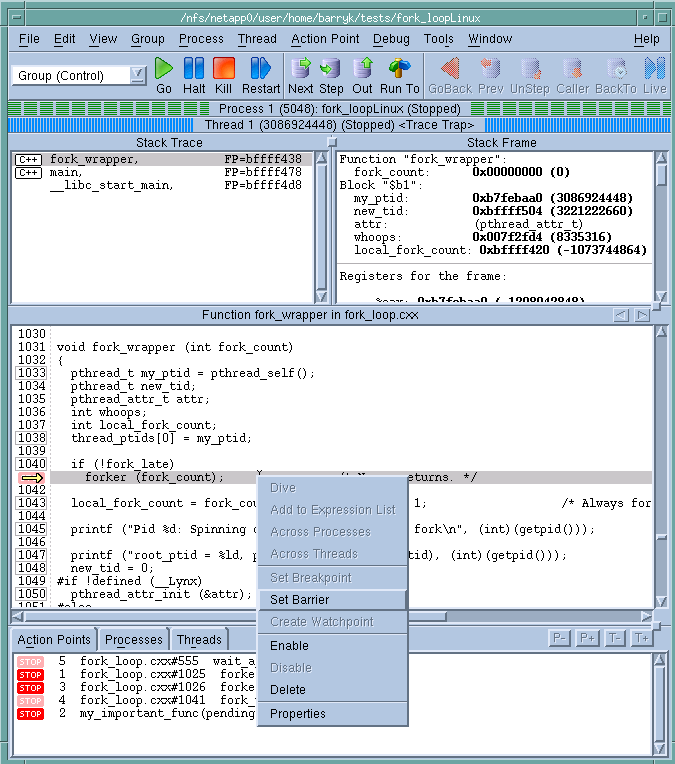
\includegraphics[height=0.75\textheight]{totalview-screenshot.png}

  \weblink{http://www.totalviewtech.com/products/totalview.html?via=rightbox}{TotalView}
  (Proprietary)
  \end{center}
\end{frame}
% -----------------------------------------------------------------------------
\begin{frame}{MPI Debuggers: DDT}
  \begin{center}
  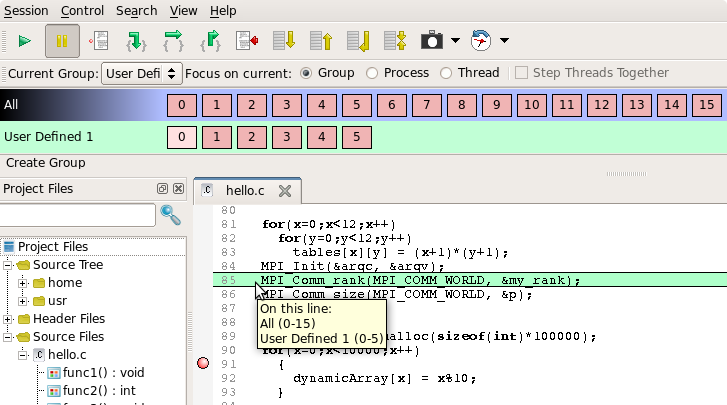
\includegraphics[width=\textwidth]{ddt-screenshot.png}

  Allinea \weblink{http://www.allinea.com/}{Distributed Debugging Tool}
  (Proprietary)
  \end{center}
\end{frame}
% -----------------------------------------------------------------------------
\begin{frame}{MPE/Jumpshot}
  \begin{center}
  \Huge MPE demo time
  \end{center}
\end{frame}
% }}}
% -----------------------------------------------------------------------------
\long\def\sectionslide#1#2#3#4{
  \begin{frame}
    \begin{center}
      {\Huge \textless #1
      {\fontsize{130}{150}\fontfamily{phv}\selectfont #2}
      \textgreater}

      \vspace{1.5cm}
      \textbf{#3}

      \medskip\footnotesize
      #4
    \end{center}
  \end{frame}
}
\sectionslide{/}{1}{Parallel Zoo}{}
\sectionslide{}{2}{\emph{Understanding} Computational Cost}{}
% -----------------------------------------------------------------------------
\section[Asymptotics]{Understanding performance through asymptotics}
% -----------------------------------------------------------------------------
\subsection{Work and Span}
% -----------------------------------------------------------------------------
% {{{
{
\colorlet{input}{green!30}
\colorlet{output}{red!30}
\colorlet{intermed}{blue!30}
\tikzset{
  input/.style={circle,fill=input,draw,thick,minimum height=4.5ex},
  output/.style={circle,fill=output,draw,thick,minimum height=4.5ex},
  func/.style={->,thick},
}
\begin{frame}{Key to parallelism: Dependencies}
  \begin{columns}
    \column{0.3\textwidth}
      B = f(A)\\
      C = g(B)\\
      E = f(C)\\
      F = h(C)\\
      G = g(E,F)\\
      P = p(B)\\
      Q = q(B)\\
      R = r(G,P,Q)
    \column{0.6\textwidth}
    \uncover<+->{}
    \uncover<+->{
      \begin{center}
        \input{general-dep-graph}
      \end{center}
    }
  \end{columns}
  \uncover<+->{
    \begin{tikzpicture} [overlay]
      \node [above left=1cm of current page.south east, draw,drop shadow,fill=white,
      inner xsep=0.5cm,inner ysep=0.5cm,thick, text width=0.5\textwidth]
        {
          Does this look a bit like \texttt{make}?

          \only<+->{
            \bigskip
            \texttt{make -j 5} runs in parallel (on 5 CPUs).
          }
        } ;
    \end{tikzpicture}
  }
\end{frame}
}
% -----------------------------------------------------------------------------
\begin{frame}{Thinking about Parallel Complexity}
  Let $T_P$ be the time taken on $P$ processors. Then;
  \begin{itemize}
    \item \textbf{Work / ``Work Complexity''} $T_1$

      Total number of operations necessary
    \item \textbf{Span / ``Step Complexity''} $T_\infty$

      Minimum number of steps taken if an infinite number of processors are available
    \item \textbf{Parallelism} $T_1/T_\infty$

      Average amount of work along span
  \end{itemize}
  \uncover<+->{}
  \uncover<+->{
    \begin{tikzpicture} [overlay]
      \node [above left=1cm of current page.south east, draw,drop shadow,fill=white,
      inner xsep=0.5cm,inner ysep=0.5cm,thick]
        {
          Does $P>T_1/T_\infty$ make sense?
        } ;
    \end{tikzpicture}
  }
\end{frame}
% -----------------------------------------------------------------------------
\begin{frame}{Work/Span: Examples}
  Determine $T_1$ and $T_\infty$ for:

  \begin{itemize}[<+->]
    \item Adding two vectors of length $n$
    \item Matrix-vector multiplication ($n \times n$)
    \item Summing a vector of length $n$
    \item \strut\only<.>{Bubble sort}\only<+->{\sout{Bubble sort} Odd-even
      transposition sort}
  \end{itemize}
\end{frame}
% -----------------------------------------------------------------------------
% }}}
% -----------------------------------------------------------------------------
\subsection{Memory Cost}
% -----------------------------------------------------------------------------
% {{{
\begin{frame}{Memory Cost by Example: Matrix Multiplication }
  \begin{columns}
    \column{0.3\textwidth}
      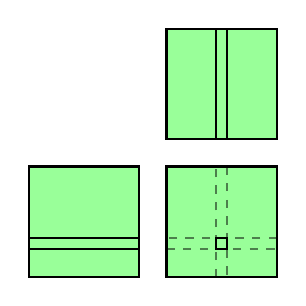
\begin{tikzpicture}[scale=0.7,
      mat/.style={draw,thick,fill=green!40},
      ]
        \path [mat] (0,0) coordinate (C) rectangle +(2,2)
          coordinate [pos=0.5] (Cmid)
          ;
        \path [mat] (C) ++(-2.5,0) coordinate (A) rectangle +(2,2)
          coordinate [pos=0.5] (Amid)
          ;
        \path [mat] (C) ++(0,2.5) coordinate (B) rectangle +(2,2)
          coordinate [pos=0.5] (Bmid)
          ;
        \draw [thick] (A) ++(0,0.5) -- ++(2,0) ++(0,0.2) -- ++(-2,0);
        \draw [thick] (B) ++(0.9,0) -- ++(0,2) ++(0.2,0) -- ++(0,-2);

        \draw [thick,dashed,opacity=0.5]
          (C) ++(0,0.5) -- ++(2,0) ++(0,0.2) -- ++(-2,0);
        \draw [thick,dashed,opacity=0.5]
          (C) ++(0.9,0) -- ++(0,2) ++(0.2,0) -- ++(0,-2);

        \draw [thick] (C) ++(0.9,0.5) rectangle ++(0.2,0.2);
      \end{tikzpicture}
    \column{0.7\textwidth}
      \uncover<+->{
        Floating Point operations: $2N^3$
      }

      \bigskip
      \uncover<+->{\emph{Inherent} data motions:}
      \uncover<+->{$3N^2$}

      \bigskip
      \uncover<+->{
      \emph{Inherent} computational intensity:
        \[
        \frac{\text{\# flops}}{\text{\# data motions}}
        = \frac{2N^3}{3N^2}
        \sim
        N
        \]
      }

      \bigskip
      \uncover<+->{
        \emph{Achieved} computational intensity (triple loops):
        \[
        \frac{\text{\# flops}}{\text{\# data motions}}
        = \frac{2N^3}{2N^3+O(N^2)}
        \sim
        1
        \]
      }
  \end{columns}
  \uncover<+->{
    \begin{tikzpicture} [overlay]
      \node [above left=1cm of current page.south east, draw,drop shadow,fill=white,
      inner xsep=0.5cm,inner ysep=0.5cm,thick, text width=0.7\textwidth]
        {
          Motion: Implies a notion of ``close'' and ``far away''.

          \bigskip
          What's ``good''? High CI? Low CI?

          \only<+->{
            \bigskip
            ``Moral CI'': Unachievable. Why?
          }

          \only<+->{
            \bigskip
            \textbf{So, what to do?}
          }
        } ;
    \end{tikzpicture}
  }
\end{frame}

\begin{frame}{Rearranging Matrix-Matrix Multiplication }
  Matrix Multiplication:
  \[
    C_{ij} = \sum_{k} A_{ik} B_{kj}
  \]
  \begin{center}
  \begin{tikzpicture}[
    mat/.style={draw,thick,fill=green!40},
    scale=0.8,
    ]
    \path [mat] (0,0) coordinate (C) rectangle +(2,2)
      coordinate [pos=0.5] (Cmid)
      ;
    \path [mat] (C) ++(-2.5,0) coordinate (A) rectangle +(2,2)
      coordinate [pos=0.5] (Amid)
      ;
    \path [mat] (C) ++(0,2.5) coordinate (B) rectangle +(2,2)
      coordinate [pos=0.5] (Bmid)
      ;
    \only<+>{
      \node at (Amid) {A};
      \node at (Bmid) {B};
      \node at (Cmid) {C};
    }
    \only<+>{
      \draw [thick] (A) ++(0,0.5) -- ++(2,0) ++(0,0.2) -- ++(-2,0);
      \draw [thick] (B) ++(0.9,0) -- ++(0,2) ++(0.2,0) -- ++(0,-2);

      \draw [thick,dashed,opacity=0.5]
        (C) ++(0,0.5) -- ++(2,0) ++(0,0.2) -- ++(-2,0);
      \draw [thick,dashed,opacity=0.5]
        (C) ++(0.9,0) -- ++(0,2) ++(0.2,0) -- ++(0,-2);

      \draw [thick] (C) ++(0.9,0.5) rectangle ++(0.2,0.2);
    }
    \only<+->{
      \draw [thick] (A) ++(0,0.5) -- ++(2,0) ++(0,0.5) -- ++(-2,0);
      \draw [thick] (B) ++(1,0) -- ++(0,2) ++(0.5,0) -- ++(0,-2);

      \draw [thick,dashed,opacity=0.5]
        (C) ++(0,0.5) -- ++(2,0) ++(0,0.5) -- ++(-2,0);
      \draw [thick,dashed,opacity=0.5]
        (C) ++(1,0) -- ++(0,2) ++(0.5,0) -- ++(0,-2);

      \only<.>{
        \fill [black,opacity=0.3]
          (A) ++(0,0.5) rectangle ++(0.5,0.5) ;
        \fill [black,opacity=0.3]
          (B) ++(1,1.5) rectangle ++(0.5,0.5) ;
        \fill [black,opacity=0.1] (C) ++(1,0.5) rectangle ++(0.5,0.5);
      }
      \only<+>{
        \fill [black,opacity=0.3]
          (A) ++(0.5,0.5) rectangle ++(0.5,0.5) ;
        \fill [black,opacity=0.3]
          (B) ++(1,1.0) rectangle ++(0.5,0.5) ;
        \fill [black,opacity=0.2] (C) ++(1,0.5) rectangle ++(0.5,0.5);
      }
      \only<+>{
        \fill [black,opacity=0.3]
          (A) ++(1,0.5) rectangle ++(0.5,0.5) ;
        \fill [black,opacity=0.3]
          (B) ++(1,0.5) rectangle ++(0.5,0.5) ;
        \fill [black,opacity=0.3] (C) ++(1,0.5) rectangle ++(0.5,0.5);
      }
      \only<+>{
        \fill [black,opacity=0.3]
          (A) ++(1.5,0.5) rectangle ++(0.5,0.5) ;
        \fill [black,opacity=0.3]
          (B) ++(1,0) rectangle ++(0.5,0.5) ;
        \fill [black,opacity=0.5] (C) ++(1,0.5) rectangle ++(0.5,0.5);
      }

      \draw [thick] (C) ++(1,0.5) rectangle ++(0.5,0.5);
    }
  \end{tikzpicture}
  \end{center}
\end{frame}
% }}}
% -----------------------------------------------------------------------------
\subsection{Pebbles and I/O}
% -----------------------------------------------------------------------------
% {{{
{
\def\depdag{
  \node [dagnode] (A) at (152,479) {A};
  \node [dagnode] (C) at (80,295) {C};
  \node [dagnode] (B) at (152,387) {B};
  \node [dagnode] (E) at (27,203) {E};
  \node [dagnode] (G) at (99,111) {G};
  \node [dagnode] (F) at (99,203) {F};
  \node [dagnode] (Q) at (211,203) {Q};
  \node [dagnode] (P) at (145,295) {P};
  \node [dagnode] (R) at (170,111) {R};
  \node [dagnode] (S) at (130,19) {S};
  \draw [->] (C) -- (F);
  \draw [->] (B) -- (C);
  \draw [->] (P) -- (R);
  \draw [->] (P) -- (E);
  \draw [->] (P) -- (F);
  \draw [->] (E) -- (G);
  \draw [->] (Q) -- (R);
  \draw [->] (F) -- (G);
  \draw [->] (B) -- (Q);
  \draw [->] (A) -- (B);
  \draw [->] (B) -- (P);
  \draw [->] (C) -- (E);
  \draw [->] (C) ..controls +(-30:50cm) and +(110:50cm).. (R);
  \draw [->] (G) -- (S);
  \draw [->] (R) -- (S);
}
\def\compute#1{
  \uncover<+->{ \node [inmem] at (#1) {#1}; }
}
\def\delete#1{
  \uncover<+->{ \node [dagnode] at (#1) {#1}; }
}
\def\bringin#1{
  \uncover<+->{ \node [inmem] at (#1) {#1}; }
}
\def\evict#1{
  \uncover<+->{ \node [far] at (#1) {#1}; }
}
\begin{frame}{How much memory is needed?}
  How much memory do we need to evaluate this DAG?
  \begin{center}
    \begin{tikzpicture}[
      scale=0.014,thick,
      dagnode/.style={circle,draw,thick,minimum
      height=4.5ex,fill=black!10},
      inmem/.style={dagnode,fill=red!30},
      ]
        \depdag

        \compute A
        \compute B
        \delete A
        \compute C

        \compute P
        \compute E
        \compute F
        \compute G
        \delete E
        \delete F

        \compute Q
        \delete B

        \compute R
        \delete C
        \delete P
        \delete Q

        \compute S
        \delete G
        \delete R

    \end{tikzpicture}
  \end{center}
  \uncover<+->{
    \begin{tikzpicture} [overlay]
      \node [above left=1cm of current page.south east, draw,drop shadow,fill=white,
      inner xsep=0.5cm,inner ysep=0.5cm,thick, text width=0.8\textwidth]
        {
          How many `memory cells' needed?
          \only<+->{\textbf{6}}

          \only<+>{
          \medskip
          What if nodes were repeatable?

          \phantom{(Interesting, but not now.)}
          }
          \only<+->{
          \medskip
          \sout{What if nodes were repeatable?}

          (Interesting, but not now.)}

          \only<+->{
          \medskip
          What if we only had 4 cells \emph{near} the processor?
          }
        } ;
    \end{tikzpicture}
  }
\end{frame}
% -----------------------------------------------------------------------------
\begin{frame}{Modeling local/\emph{close} memory}
  Rules, each with unit cost:
  \bigskip
  \begin{description}
    \item[Compute] If all inputs of a pebble are red, color the pebble
    red.
    \item[Delete] Remove a pebble from the board.
    \item[Evict] Turn a red pebble into a blue pebble.
    \item[Bring close] Turn a blue pebble into a red pebble.
  \end{description}
  \creditto{Hong \& Kung `81}
\end{frame}
% -----------------------------------------------------------------------------
\begin{frame}{Turning Non-local Storage into Cost}
  How long does it take to evaluate this DAG with only 4 `red pebbles'
  (`close' memory cells)?
  \begin{center}
    \begin{tikzpicture}[
      scale=0.014,thick,
      dagnode/.style={circle,draw,thick,minimum
      height=4.5ex,fill=black!10},
      inmem/.style={dagnode,fill=red!30},
      far/.style={dagnode,fill=blue!30},
      ]
        \depdag

        \compute A
        \compute B
        \delete A
        \compute C

        \compute P
        \compute E
        \evict B
        \compute F
        \evict C
        \compute G
        \delete E
        \delete F

        \bringin B
        \compute Q
        \delete B
        \bringin C
        \evict G
        \compute R

        \delete C
        \delete P
        \delete Q
        \bringin G
        \compute S

        \delete G
        \delete R
    \end{tikzpicture}
  \end{center}
  \begin{tikzpicture} [overlay]
    \node [above right=2cm and 1cm of current page.south west, draw,fill=white,
    inner xsep=0.5cm,inner ysep=0.5cm,thick]
      {
        \overlaynumber
      } ;
  \end{tikzpicture}

  \creditto{Hong \& Kung `81}
\end{frame}
}
% -----------------------------------------------------------------------------
\begin{frame}{Red/Blue Pebbles: Theory}
  Examples of theoretical results from [Hong, Kung `81]:

  \bigskip
  Matrix-vector Multiplication:
  \[
    \text{Min I/O time}\sim \frac{n^2}{\text{\# close cells}}
  \]

  \bigskip
  Matrix-matrix Multiplication:
  \[
    \text{Min I/O time}\sim \frac{n^3}{\sqrt{\text{\# close cells}}
    }
  \]
\end{frame}

\begin{frame}{Red/Blue Pebbles: Theory}
  Fast Fourier Transform:
  \begin{center}
    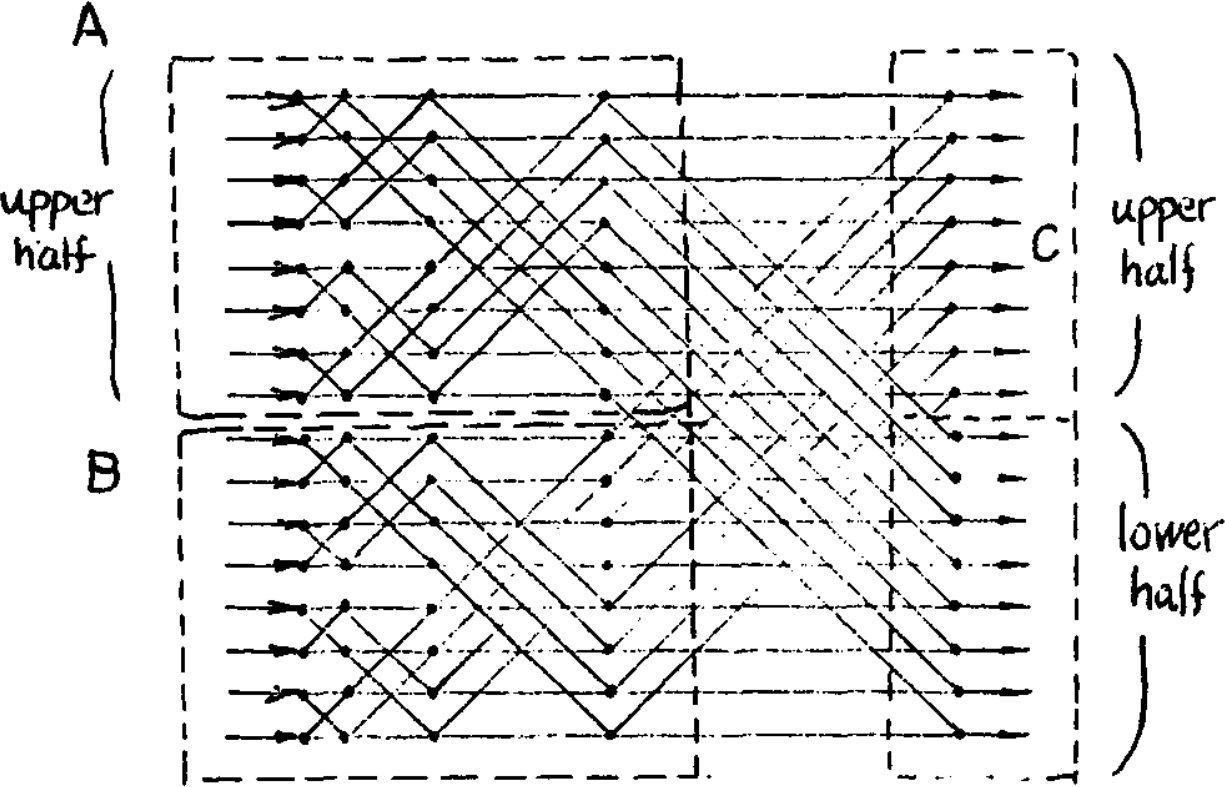
\includegraphics[width=5cm]{hong-kung-fft.png}
  \end{center}
  \[
    \text{Min I/O time}\sim \frac{n \log n}{\log \text{\# close cells}}
  \]
\end{frame}
% }}}
% -----------------------------------------------------------------------------
\section{Closer to the machine}
% -----------------------------------------------------------------------------
% {{{
\begin{frame}{Taking a step back}
  \begin{center}
  \textbf{Want to answer:}

  \emph{How fast} does a computer execute my code?

  \bigskip
  \textbf{Need to answer first:}

  \emph{How} does a computer execute my code?
  \end{center}
\end{frame}
% -----------------------------------------------------------------------------
\begin{frame}{What's in a computer?}
  \begin{center}
  \tikz \node (board) {
  \includegraphics[width=0.8\textwidth]{mainboard.jpeg}
  } ;
  \end{center}

  \tikz \coordinate (cpu) at ($ (board.south east)+(-1,3.5) $) ;
  \tikz \coordinate (mem) at ($ (board.south east)+(-2,1) $) ;
  \tikz \coordinate (pci) at ($ (board.north west)+(2,-3.5) $) ;

  \uncover<+>{}
  \uncover<+-+(1)>{
    \begin{tikzpicture} [overlay]
      \node [left=2cm of cpu,rectangle callout,draw,thick,
        callout absolute pointer=(cpu),xshift=-0.4cm,
        callout pointer shorten=1cm,text width=6cm,
        fill=white,drop shadow,inner sep=3mm]
        {
          Processor

          \medskip
          \tikz \node (substrate) [inner sep=0] {
          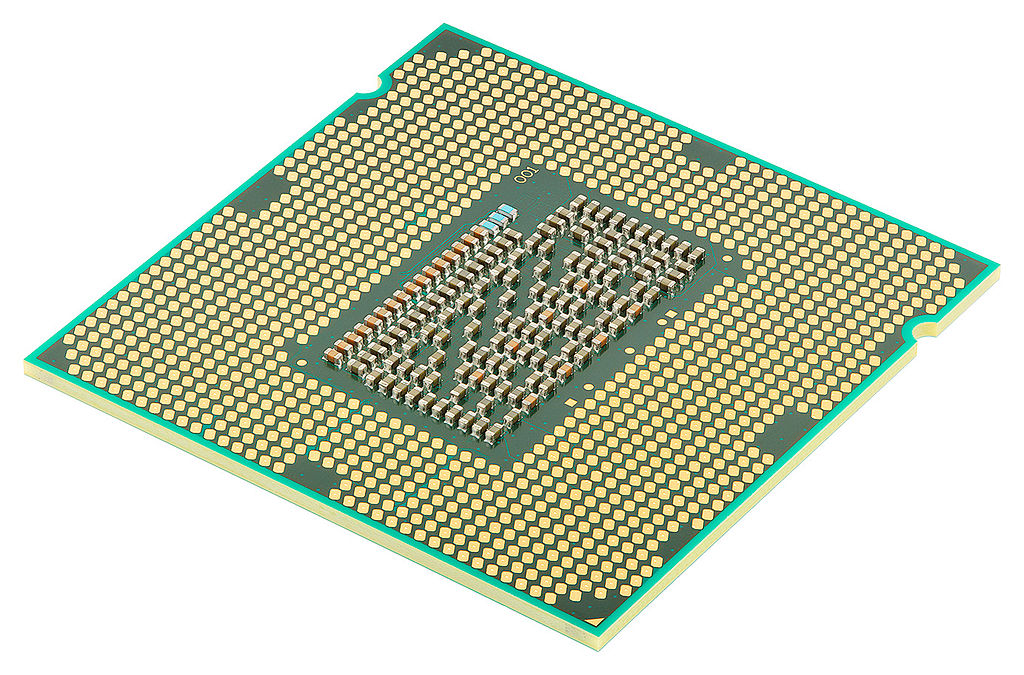
\includegraphics[width=\textwidth]{sandy-bridge-bottom.jpeg}
          } ;
          Intel Core i7-2620M, 2.7 GHz

          ``Sandy bridge'' $\mu$arch
        };
    \end{tikzpicture}
  }

  \uncover<+>{
    \begin{tikzpicture} [overlay]
      \node [right=-0.5cm of substrate,rectangle callout,draw,thick,
        callout absolute pointer=(substrate),yshift=1.5cm, text width=4cm,
        fill=white,drop shadow,inner sep=3mm]
        {
          Die

          \medskip
          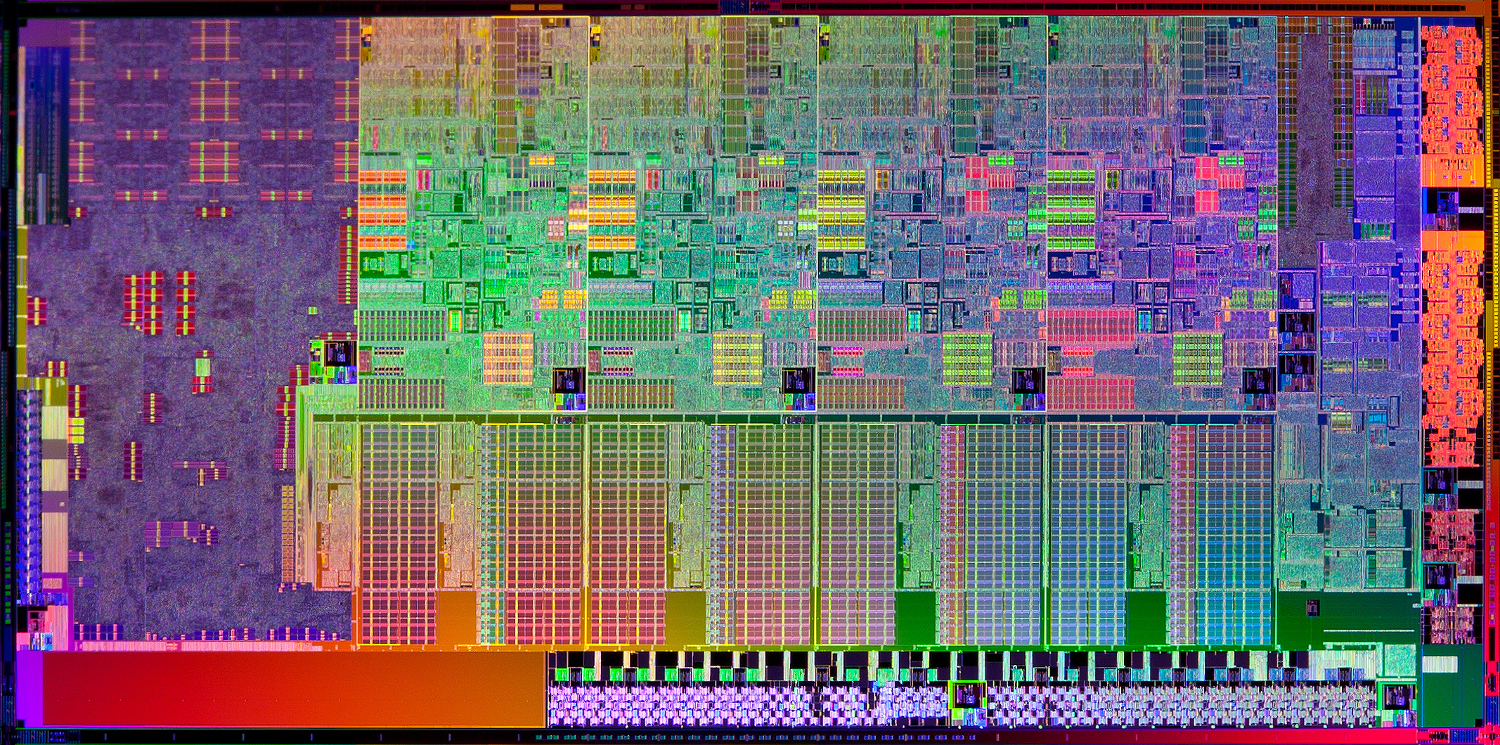
\includegraphics[width=5cm,angle=90]{sandy-bridge-die-shot.jpeg}

          149 mm${}^2$, 2 real cores

          624,000,000 transistors

          $\sim$ 35W
        };
    \end{tikzpicture}
  }

  \uncover<+>{}
  \uncover<+>{
    \begin{tikzpicture} [overlay]
      \node [above=2cm of mem,rectangle callout,draw,thick,
        callout absolute pointer=(mem),xshift=-0.4cm,
        callout pointer shorten=1cm,text width=4cm,
        fill=white,drop shadow,inner sep=3mm]
        {
          Memory

          \includegraphics[width=\textwidth]{memory.png}
        };
    \end{tikzpicture}
  }

  \uncover<+>{}
  \uncover<+-+(1)>{
    \begin{tikzpicture} [overlay]
      \node [right=1.5cm of pci,rectangle callout,draw,thick,
        callout absolute pointer=(pci),xshift=-0.4cm,
        callout pointer shorten=0.3cm,text width=5cm,
        fill=white,drop shadow,inner sep=5mm]
        (expansion-slots)
        {
          Expansion Slots

          \medskip
          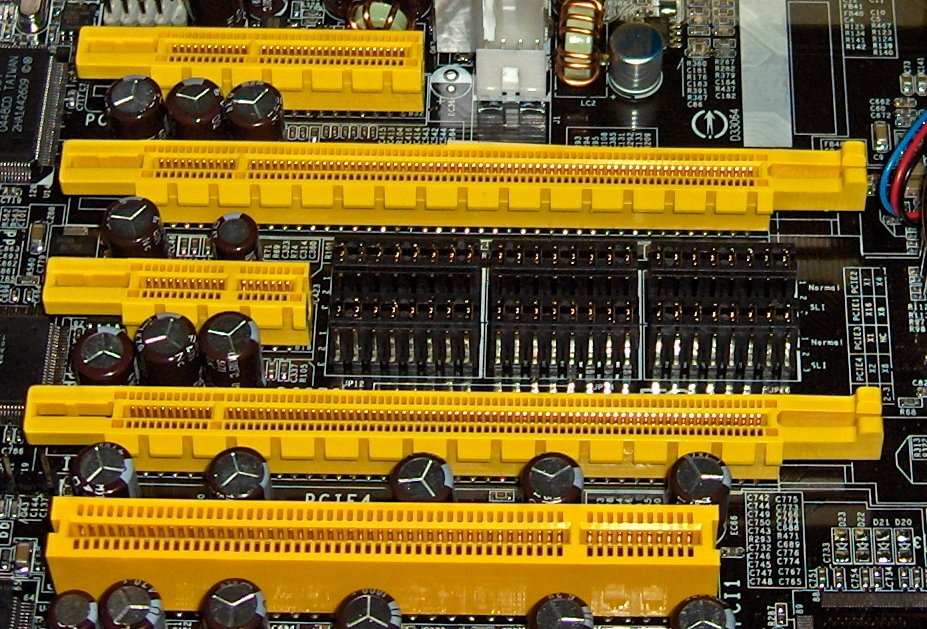
\includegraphics[height=3cm]{pci-express.jpeg}

          \medskip
          PCI-Express (x4, x16, x1, x16) and regular PCI

          \medskip
          PCIe V2, x16 Bandwidth:\\
          $\sim$ 6 GB/s
        };
    \end{tikzpicture}
  }
  \tikz \coordinate (pciex-slot) at ($ (expansion-slots.north west)+(2,-1.5) $) ;

  \uncover<+>{
    \begin{tikzpicture} [overlay]
      \node [below=1.5cm of pciex-slot,rectangle callout,draw,thick,
        callout absolute pointer=(pciex-slot),xshift=-0.4cm,
        callout pointer shorten=0.5cm,text width=4cm,
        fill=white,drop shadow,inner sep=3mm]
        {
          \includegraphics[width=\textwidth]{gtx480.png}

          GPU goes here
        };
    \end{tikzpicture}
  }
  \uncover<+>{}

\end{frame}
\addimgcredit{ Mainboard: Wikimedia Commons \cc}
\addimgcredit{ PCI Express slots: Wikimedia Commons \cc}
\addimgcredit{ DIMM: sxc.hu/gobran11 }
\addimgcredit{ Sandy bridge bottom: Wikimedia Commons \cc }
\addimgcredit{ Sandy bridge die: Intel Corp. }
\addimgcredit{ GTX 480: Nvidia Corp. \cc}
% }}}
% -----------------------------------------------------------------------------
\subsection[Basics]{The Basic Subsystems}
% -----------------------------------------------------------------------------
% {{{
\def\procpic{
  \node [rectangle,draw,thick,fill=green!30, inner xsep=4cm,
    anchor=south] at (0,0) (idbus) { Internal Bus };
  \node (reg) [rectangle,draw,thick,fill=black!20,
    inner ysep=5mm,anchor=south]
    at ($ (idbus.north) + (-2cm,0.75) $) {Register File} ;
  \node (flags) [anchor=south east,draw,thick,fill=black!20,inner ysep=0.75mm]
    at(reg.south east) {Flags} ;
  \node (alu) [trapezium,
    trapezium left angle=130,
    trapezium right angle=130,
    inner ysep=3mm,
    draw,thick,fill=black!20,anchor=north]
    at ($ (idbus.south) + (2,-0.75) $) {Data ALU} ;
  \node (addr) [trapezium,
    trapezium left angle=50,
    trapezium right angle=50,
    inner ysep=3mm,
    draw,thick,fill=black!20,anchor=south west]
    at ($ (reg.north) + (0,0.75) $) {Address ALU} ;
  \node (ctrl) [arrow box,draw,thick,fill=black!20,anchor=north,
    inner ysep=5mm,arrow box arrows={north:.475cm,east:.475cm},
    arrow box shaft width=2mm,inner xsep=4mm]
    at ($ (idbus.south) + (-2cm,-0.275) $) {Control Unit} ;
  \node (pc) [anchor=north east,draw,thick,fill=black!20,inner ysep=0.75mm]
    at(ctrl.north east) {PC} ;
  \node (mem) [rectangle,draw,thick,fill=black!20,
    inner ysep=3mm,anchor=west,rotate=90,inner xsep=5mm,minimum
    width=3.5cm, minimum height=1cm]
    at ($ (idbus.north) + (2,0.75) $) { } ;
  \node at (mem.south east) [anchor=north west] {Memory Interface} ;
  \draw [line width=1mm,<-] (alu.north west) -- +(0,0.75) ;
  \draw [line width=1mm,<-] (alu.north east) -- +(0,0.75) ;
  \draw [line width=1mm,->] (alu.south) |- +(1,-0.25) -| ($ (idbus.south) + (4.5,0) $);
  \draw [line width=1mm,<->] (reg.south) -- +(0,-0.75);
  \draw [line width=1mm,->] (reg.north) -- (addr.south west);
  \draw [line width=1mm,->] ($ (idbus.north) + (-0.5,0) $) |- ++(0,2.5) -| (addr.south east);
  \draw [line width=1mm,->] ($ (idbus.south) + (-4,0) $) |- (ctrl.west)
    node [pos=0.3,anchor=east,font=\footnotesize,text width=7mm] {Insn. fetch};
  \draw [line width=1mm,->] (addr.north) |- ++(2.6,0.25) |- (mem.north) ;
  \draw [line width=1mm,<->] (mem.west) -- +(0,-0.75) ;
  \draw [line width=1mm,<->] (mem.west) -- +(0,-0.75) ;
  \draw [line width=1mm,<->] (mem.west) -- +(0,-0.75) ;
  \draw [line width=1mm,<->] ($ (mem.south) + (0,-.75) $) coordinate (dataexit) -- +(0.75,0)
    node [pos=1,anchor=west] {Data Bus} ;
  \draw [line width=1mm,->] ($ (mem.south) + (0,.75) $) coordinate (addrexit) -- +(0.75,0)
    node [pos=1,anchor=west] {Address Bus} ;

  \draw [line width=1mm,dotted,opacity=0.3] (dataexit) -| (mem.west) ;
  \draw [line width=1mm,dotted,opacity=0.3] (addrexit) -| ++(-0.4,0) |- (mem.north) ;
}
\begin{frame}{A Basic Processor}
  \begin{tikzpicture}
    \procpic
  \end{tikzpicture}
  {\small (loosely based on Intel 8086)}
  \uncover<2>{
    \begin{tikzpicture} [overlay]
      \node [draw,drop shadow,fill=white,anchor=south west,xshift=1cm,yshift=1.5cm,
      text width=0.4\textwidth, inner xsep=0.5cm,inner ysep=0.5cm,thick]
        at (current page.south west)
        {
        \emph{Bonus Question:}

        What's a
        \weblink{http://en.wikipedia.org/wiki/Bus_(computing)}{bus}?
        } ;
    \end{tikzpicture}
  }
\end{frame}
% -----------------------------------------------------------------------------
\begin{frame}{How all of this fits together}
  \begin{columns}
    \column{0.6\textwidth}
      Everything synchronizes to the \emph{Clock}.
      \medskip

      \emph{Control Unit} (``CU''): The brains of the operation.
      Everything connects to it.
      \medskip

      Bus entries/exits are \emph{gated} and (potentially)
      \emph{buffered}.
      \medskip

      CU controls gates, tells other units about `what' and `how':
      \begin{itemize}
        \item What operation?
        \item Which register?
        \item Which addressing mode?
      \end{itemize}

    \column{0.4\textwidth}
      \begin{tikzpicture}
        \begin{scope}[transform canvas={scale=0.4}]
          \procpic
        \end{scope}
        \path [use as bounding box] (-2,-2) rectangle (2,2);
      \end{tikzpicture}

  \end{columns}
\end{frame}
% -----------------------------------------------------------------------------
\begin{frame}{What is\dots an ALU?}
  \begin{columns}
    \column{0.6\textwidth}

      \textbf{A}rithmetic \textbf{L}ogic \textbf{U}nit

      One or two operands A, B

      Operation selector (Op):
      \begin{itemize}
        \item (Integer) Addition, Subtraction
        \item (Logical) And, Or, Not
        \item (Bitwise) Shifts (equivalent to multiplication by power of
        two)
        \item (Integer) Multiplication, Division
      \end{itemize}

      Specialized ALUs:
      \begin{itemize}
        \item \weblink{http://en.wikipedia.org/wiki/Floating_point}{Floating Point} Unit (FPU)
        \item Address ALU
      \end{itemize}

      Operates on
      \weblink{http://en.wikipedia.org/wiki/Binary_number_system}{binary representations} of numbers.
      Negative numbers represented by
      \weblink{http://en.wikipedia.org/wiki/Two's_complement}{two's
      complement}.
    \column{0.4\textwidth}
      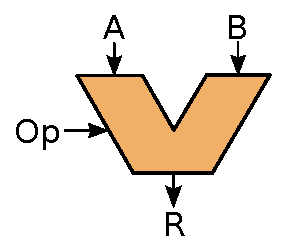
\includegraphics[width=\textwidth]{alu.pdf}
  \end{columns}
\end{frame}
% -----------------------------------------------------------------------------
\begin{frame}{What is\dots a Register File?}
  \begin{columns}
    \column{0.7\textwidth}
      \textbf{Registers} are \emph{On-Chip Memory}

      \begin{itemize}
        \item
        Directly usable as operands in\\
        Machine Language

        \item
        Often ``general-purpose''

        \item
        Sometimes special-purpose: Floating point, Indexing,
        Accumulator

        \item
        Small: x86\_64: 16$\times$64 bit GPRs

        \item Very fast (near-zero latency)
      \end{itemize}

    \column{0.3\textwidth}
      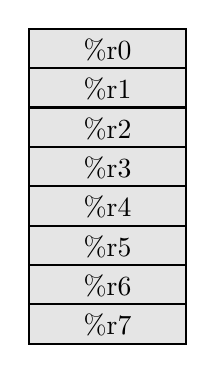
\begin{tikzpicture}
        \filldraw [gray!20,thick,draw=black] (0,0) rectangle (2,-4) ;
        \foreach \i in {0,1,...,7}
        {
          \draw [thick] (0,\i*-0.5) -- +(2,0) ;
          \node [anchor=north]  at (1,\i*-0.5) {\%r\i };
        }
      \end{tikzpicture}
  \end{columns}
  \uncover<+>{}
  \uncover<+>{
    \begin{tikzpicture} [overlay]
      \node [above left=1cm of current page.south east, draw,drop shadow,fill=white,
      inner xsep=0.5cm,inner ysep=0.5cm,thick]
        {
          First red/blue pebble game, played by compiler.
        } ;
    \end{tikzpicture}
  }
\end{frame}
% -----------------------------------------------------------------------------
\input{how-does-computer-memory-work}
\begin{frame}{What is\dots a Memory Interface?}
  \begin{columns}
    \column{0.7\textwidth}
      \textbf{Memory Interface} gets and stores binary words in
      off-chip memory.
      \medskip

      Smallest granularity: Bus width
      \medskip

      Tells outside memory
      \begin{itemize}
        \item ``where'' through \emph{address bus}
        \item ``what'' through \emph{data bus}
      \end{itemize}

      Computer main memory is ``Dynamic RAM''
      (\weblink{http://en.wikipedia.org/wiki/Dynamic_random_access_memory}{DRAM}):
      Slow, but small and cheap.

    \column{0.3\textwidth}
      \includegraphics[width=\textwidth]{memory.png}
  \end{columns}
\end{frame}
% }}}
% -----------------------------------------------------------------------------
\subsection[Assembly]{Machine Language}
% -----------------------------------------------------------------------------
% {{{
\begin{frame}[fragile]{A Very Simple Program}
  \begin{columns}
    \column{0.25\textwidth}
    \lstinputlisting[linerange=start-end]{assembly.c}
    \column{0.75\textwidth}
    \lstinputlisting[language=HTML,basicstyle=\footnotesize]{assembly.S}
  \end{columns}

  Things to know:
  \begin{itemize}
  \item \weblink{http://en.wikipedia.org/wiki/Addressing_mode}{Addressing
  modes} (Immediate, Register, Base plus Offset)
  \item
  \weblink{http://en.wikipedia.org/wiki/Hexadecimal}{0xHexadecimal}
  \item ``AT\&T Form'': (we'll use this)\\
    \verb|<opcode><size> <source>, <dest>|
  \end{itemize}
\end{frame}
\begin{frame}{Another Look}
  \begin{tikzpicture}
    \procpic
  \end{tikzpicture}
  \uncover<2>{
  \begin{tikzpicture} [overlay]
    \node [draw,drop shadow,fill=white,anchor=north east,xshift=-0.5cm,yshift=-0.5cm,
    text width=0.6\textwidth, inner ysep=1mm,thick,inner xsep=3mm]
      at (current page.north east)
      {
        \lstinputlisting[language=HTML,basicstyle=\tiny]{assembly.S}
      } ;
  \end{tikzpicture}
  }
\end{frame}
\begin{frame}[fragile]{A Very Simple Program: Intel Form}
  \lstinputlisting[language=HTML,basicstyle=\footnotesize]{assembly-intel.S}

  \begin{itemize}
  \item ``Intel Form'': (you might see this on the net)\\
    \verb|<opcode> <sized dest>, <sized source>|
  \item Goal: Reading comprehension.
  \item Don't understand an opcode?\\
    Google ``\verb|<opcode> intel instruction|''.
  \end{itemize}
\end{frame}
\begin{frame}{Machine Language Loops}
  \begin{columns}
    \column{0.3\textwidth}
    \lstinputlisting{loop-assembly.c}
    \column{0.75\textwidth}
    \lstinputlisting[language=HTML,basicstyle=\scriptsize]{loop-assembly.S}
  \end{columns}

  Things to know:
  \begin{itemize}
  \item
  \weblink{http://en.wikipedia.org/wiki/Status_register}{Condition
  Codes (Flags)}: Zero, Sign, Carry, etc.
  \item \weblink{http://en.wikipedia.org/wiki/Call_stack}{Call Stack}:
    Stack frame, stack pointer, base pointer
  \item
  \weblink{http://en.wikipedia.org/wiki/Application_binary_interface}{ABI}:
    Calling conventions
  \end{itemize}

  \uncover<2>{
  \begin{tikzpicture} [overlay]
    \node [draw,drop shadow,fill=white,anchor=south east,xshift=-1cm,yshift=1cm,
    text width=0.9\textwidth,thick,inner sep=5mm]
      at (current page.south east)
      {
        \begin{itemize}
          \item DIY Demo

          \item \url{http://assembly.ynh.io/}

            [\url{https://github.com/ynh/cpp-to-assembly}]
          \item \url{http://gcc.godbolt.org/}

          \item \url{http://llvm.org/demo/}
        \end{itemize}
      } ;
  \end{tikzpicture}
  }
\end{frame}
% -----------------------------------------------------------------------------
\begin{frame}{Web demo}
  \begin{center}
  \Huge \url{http://assembly.ynh.io/} demo time
  \end{center}
\end{frame}
% -----------------------------------------------------------------------------
\begin{frame}{We know how a computer works!}

  All of this can be built in about 4000 transistors.

  (e.g. MOS 6502 in Apple II, Commodore 64, Atari 2600)
  \medskip

  So what exactly is Intel doing with the other 623,996,000 transistors?
  \medskip

  Answer: \uncover<2->{\emph{Make things go faster!}}
  \medskip

  \uncover<3->{
  \textbf{Goal now:}

  Understand sources of slowness, and how they get addressed.
  \medskip

  Remember: \emph{High Performance} Computing
  }
\end{frame}
% }}}
% -----------------------------------------------------------------------------
\subsection[Memory]{The Memory Hierarchy}
% -----------------------------------------------------------------------------
% {{{
\begin{frame}{Source of Slowness: Memory}
  Memory is slow.
  \medskip

  Distinguish two different versions of ``slow'':
  \begin{itemize}
    \item Bandwidth
    \item Latency
  \end{itemize}
  $\rightarrow$ Memory has \emph{long latency}, but can have
  \emph{large bandwidth}.

  \begin{center}
  \includegraphics[width=0.4\textwidth]{mainboard.jpeg}
  \end{center}

  Size of die vs. distance to memory: big!

  \medskip
  Dynamic RAM: long intrinsic latency!

  \uncover<2>{
    \begin{tikzpicture} [overlay]
      \node [draw,drop shadow,fill=white,anchor=south east,xshift=-0.5cm,yshift=0.5cm,
      text width=0.4\textwidth, inner sep=3mm,thick]
        at (current page.south east)
        {
        \emph{Idea:}\\[1ex]
        Put a look-up table of recently-used data onto the
        chip.\\[1ex]
        $\rightarrow$
        ``\weblink{http://en.wikipedia.org/wiki/CPU_cache}{Cache}''
        } ;
    \end{tikzpicture}
  }
\end{frame}

% -----------------------------------------------------------------------------
\begin{frame}{The Memory Hierarchy}
  Hierarchy of increasingly bigger, slower memories:

  \begin{center}
  \begin{tikzpicture}[hieblock/.style={thick,draw,fill=green!20,
  text width=0.4\textwidth, text centered}]
    \node [hieblock] (reg) {Registers};
    \node [hieblock,below=3ex of reg] (l1) {L1 Cache};
    \node [hieblock,below=3ex of l1] (l2) {L2 Cache};
    \node [hieblock,below=3ex of l2] (dram) {DRAM};
    \node [hieblock,below=3ex of dram] (virt) {Virtual Memory\\ (hard drive)};

    \node [right=2em of reg] {1 kB, 1 cycle };
    \node [right=2em of l1] {10 kB, 10 cycles };
    \node [right=2em of l2] {1 MB, 100 cycles };
    \node [right=2em of dram] {1 GB, 1000 cycles };
    \node [right=2em of virt] {1 TB, 1 M cycles };

    \draw [thick,<->] (reg) -- (l1) ;
    \draw [thick,<->] (l1) -- (l2) ;
    \draw [thick,<->] (l2) -- (dram) ;
    \draw [thick,<->] (dram) -- (virt) ;
  \end{tikzpicture}
  \end{center}
  \uncover<2>{
    \begin{tikzpicture} [overlay]
      \node [draw,drop shadow,fill=white,anchor=south east,xshift=-0.5cm,yshift=0.5cm,
      text width=0.6\textwidth, inner sep=5mm,thick]
        at (current page.south east)
        {
          Second red/blue pebble game: played by cache controller

          \bigskip
          What is a \emph{working set}?

          \bigskip
          How might \emph{data locality} factor into this?
        } ;
    \end{tikzpicture}
  }
\end{frame}

% -----------------------------------------------------------------------------
\begin{frame}{Cache: Actual Implementation}
  \begin{columns}
    \column{0.55\textwidth}
      Demands on cache implementation:
      \begin{itemize}
        \item Fast, small, cheap, low power
        \item Fine-grained
        \item High ``hit''-rate (few ``misses'')
      \end{itemize}

    \column{0.4\textwidth}
      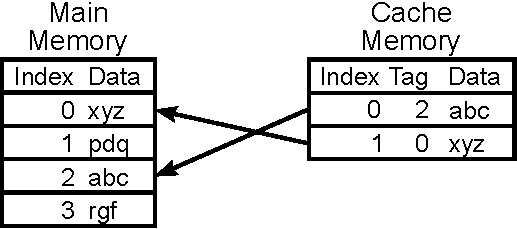
\includegraphics[width=\textwidth]{basic-cache.pdf}
  \end{columns}

  \bigskip
  \emph{Problem:}

  \colorbox{gray!20}{
  Goals at odds with each other:
  Access matching logic expensive!
  }

  \bigskip
  \emph{Solution 1}: More data per unit of access matching logic\\
  \hfill $\rightarrow$ Larger ``Cache Lines''

  \bigskip
  \emph{Solution 2}: Simpler/less access matching logic\\
  \hfill $\rightarrow$ Less than full ``Associativity''

  \bigskip
  Other choices: Eviction strategy, size
\end{frame}
\addimgcredit{Basic cache: Wikipedia \cc}
% -----------------------------------------------------------------------------
\begin{frame}{Cache: Associativity}
  \begin{center}
    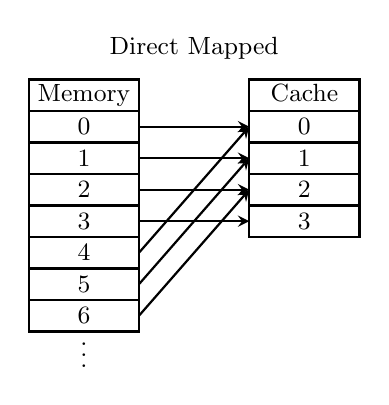
\begin{tikzpicture}[yscale=-0.4,xscale=0.7,font=\small]

      \node at (3,-2) { Direct Mapped } ;
      \draw [thick] (0,0) rectangle +(2,-1)
        node [pos=0.5,text depth=0.4ex] {Memory};
      \foreach\i in {0,1,2,...,6}
      {
        \draw [thick] (0,\i) rectangle +(2,1) node [pos=0.5] {\i};
        \pgfmathtruncatemacro{\tgt}{mod(\i,4)}
        \draw [-stealth,thick] (2,\i+0.5) -- (4,\tgt+0.5) ;
      }
      \node at (1,7.5) { $\vdots$ };

      \draw [thick] (4,0) rectangle +(2,-1)
        node [pos=0.5,text depth=0.4ex] {Cache};
      \foreach\i in {0,1,2,...,3}
      \draw [thick] (4,\i) rectangle +(2,1) node [pos=0.5] {\i};

    \end{tikzpicture}
    \hspace{1cm}
    \uncover<+->{}
    \uncover<+->{
      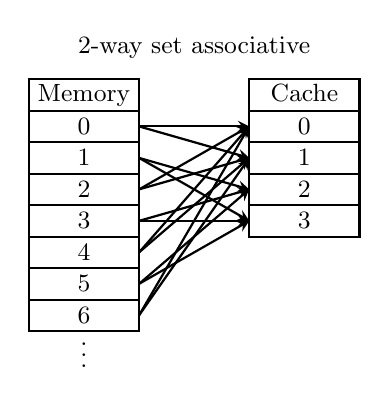
\begin{tikzpicture}[yscale=-0.4,xscale=0.7,font=\small]
        \node at (3,-2) { 2-way set associative } ;
        \draw [thick] (0,0) rectangle +(2,-1)
        node [pos=0.5,text depth=0.4ex] {Memory};
        \foreach\i in {0,1,2,...,6}
        {
          \draw [thick] (0,\i) rectangle +(2,1) node [pos=0.5] {\i};
          \pgfmathtruncatemacro{\tgt}{mod(2*\i,4)}
          \draw [-stealth,thick] (2,\i+0.5) -- (4,\tgt+0.5) ;
          \uncover<+->{
            \pgfmathtruncatemacro{\tgt}{mod(2*\i+1,4)}
            \draw [-stealth,thick] (2,\i+0.5) -- (4,\tgt+0.5) ;
          }
        }
        \node at (1,7.5) { $\vdots$ };

        \draw [thick] (4,0) rectangle +(2,-1)
        node [pos=0.5,text depth=0.4ex] {Cache};
        \foreach\i in {0,1,2,...,3}
        \draw [thick] (4,\i) rectangle +(2,1) node [pos=0.5] {\i};

      \end{tikzpicture}
    }
  \end{center}
  \uncover<+>{
  \begin{tikzpicture} [overlay]
    \node [draw,drop shadow,fill=white,anchor=south east,xshift=-1cm,yshift=1cm,
    text width=0.7\textwidth,thick,inner sep=5mm]
      at (current page.south east)
      {
        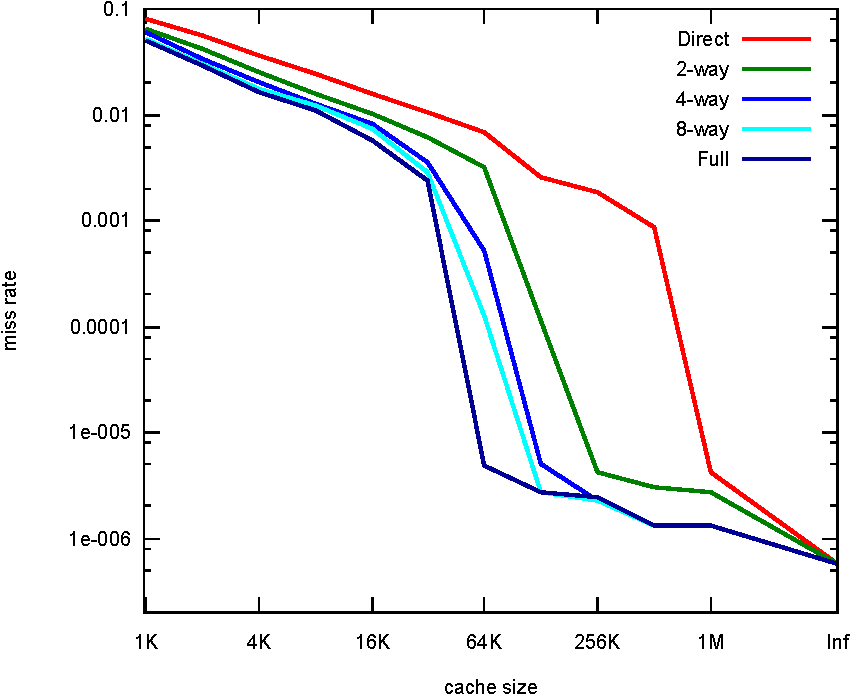
\includegraphics[width=\textwidth]{cache-assoc-miss.pdf}

        Miss rate versus cache size on the Integer portion of
        SPEC~CPU2000 [Cantin, Hill 2003]
      } ;
  \end{tikzpicture}
  }
\end{frame}
\addimgcredit{Cache associativity: based on Wikipedia \cc}
\addimgcredit{Cache associativity vs miss rate: Wikipedia \cc, }

% -----------------------------------------------------------------------------
\begin{frame}{CPUID}
  \begin{center}
  \Huge CPUID demo time
  \end{center}
\end{frame}

\def\cacheslide#1#2{
\begin{frame}{#1}
  \lstinputlisting[basicstyle=\scriptsize]{microbench/#2.c}
  \creditto{Original benchmarks by Igor Ostrovsky}
  \uncover<2>{
    \begin{tikzpicture} [overlay]
      \node [draw,drop shadow,fill=white,anchor=south east,xshift=-0.5cm,yshift=0.5cm,
      text width=0.8\textwidth, inner sep=5mm,thick]
        at (current page.south east)
        {
        \includegraphics[width=\textwidth]{microbench/#2-crop.pdf}
        } ;
    \end{tikzpicture}
  }
\end{frame}
}

\cacheslide{Updating every $k$th integer}{strides}
\cacheslide{Measuring bandwidths}{bw}
\cacheslide{Another mystery}{assoc}

\addimgcredit{Cache Measurements: Igor Ostrovsky}

% -----------------------------------------------------------------------------
\begin{frame}{Core Message}
  \begin{center}
    Learned a lot about caches.

    \bigskip
    Also learned:

    \bigskip
    {\Large Honest measurements are \emph{hard}.}

    \vspace{2cm}
    A good attempt:

    \url{http://www.bitmover.com/lmbench/}

    \footnotesize
    Instructions:

    \url{http://download.intel.com/design/intarch/papers/321074.pdf}
  \end{center}
\end{frame}
% -----------------------------------------------------------------------------
\begin{frame}{Programming for the Cache}
  How can we rearrange programs to be cache-friendly?

  \bigskip
  Examples:
  \begin{itemize}
  \item<+-> Large vectors $x$, $a$, $b$

  Compute\[
  x \leftarrow x+3a-5b.
  \]
  \item<+-> Matrix-Matrix Multiplication
  \end{itemize}
\end{frame}
% }}}
% -----------------------------------------------------------------------------
\subsection{Pipelines}
% -----------------------------------------------------------------------------
% {{{
\begin{frame}{Source of Slowness: Sequential Operation}
  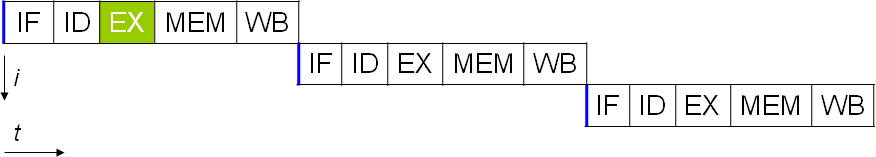
\includegraphics[width=\textwidth]{no-pipeline.png}
  \begin{description}
    \item[IF] Instruction fetch
    \item[ID] Instruction Decode
    \item[EX] Execution
    \item[MEM] Memory Read/Write
    \item[WB] Result Writeback
  \end{description}
\end{frame}
\addimgcredit{Pipelining: Wikipedia \cc}
\begin{frame}{Solution: Pipelining}
  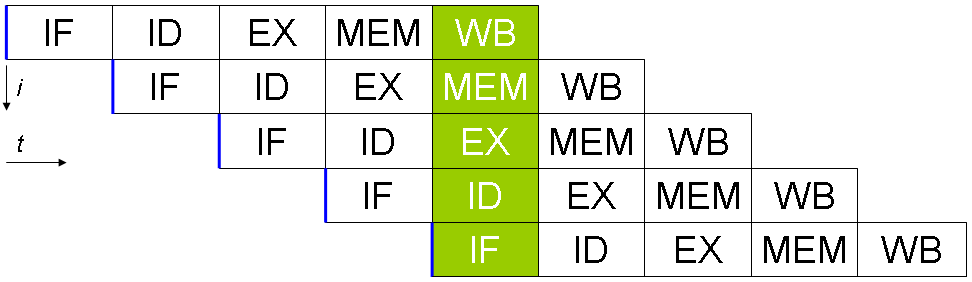
\includegraphics[width=\textwidth]{five-stage-pipeline.png}
\end{frame}
\begin{frame}{Pipelining}
  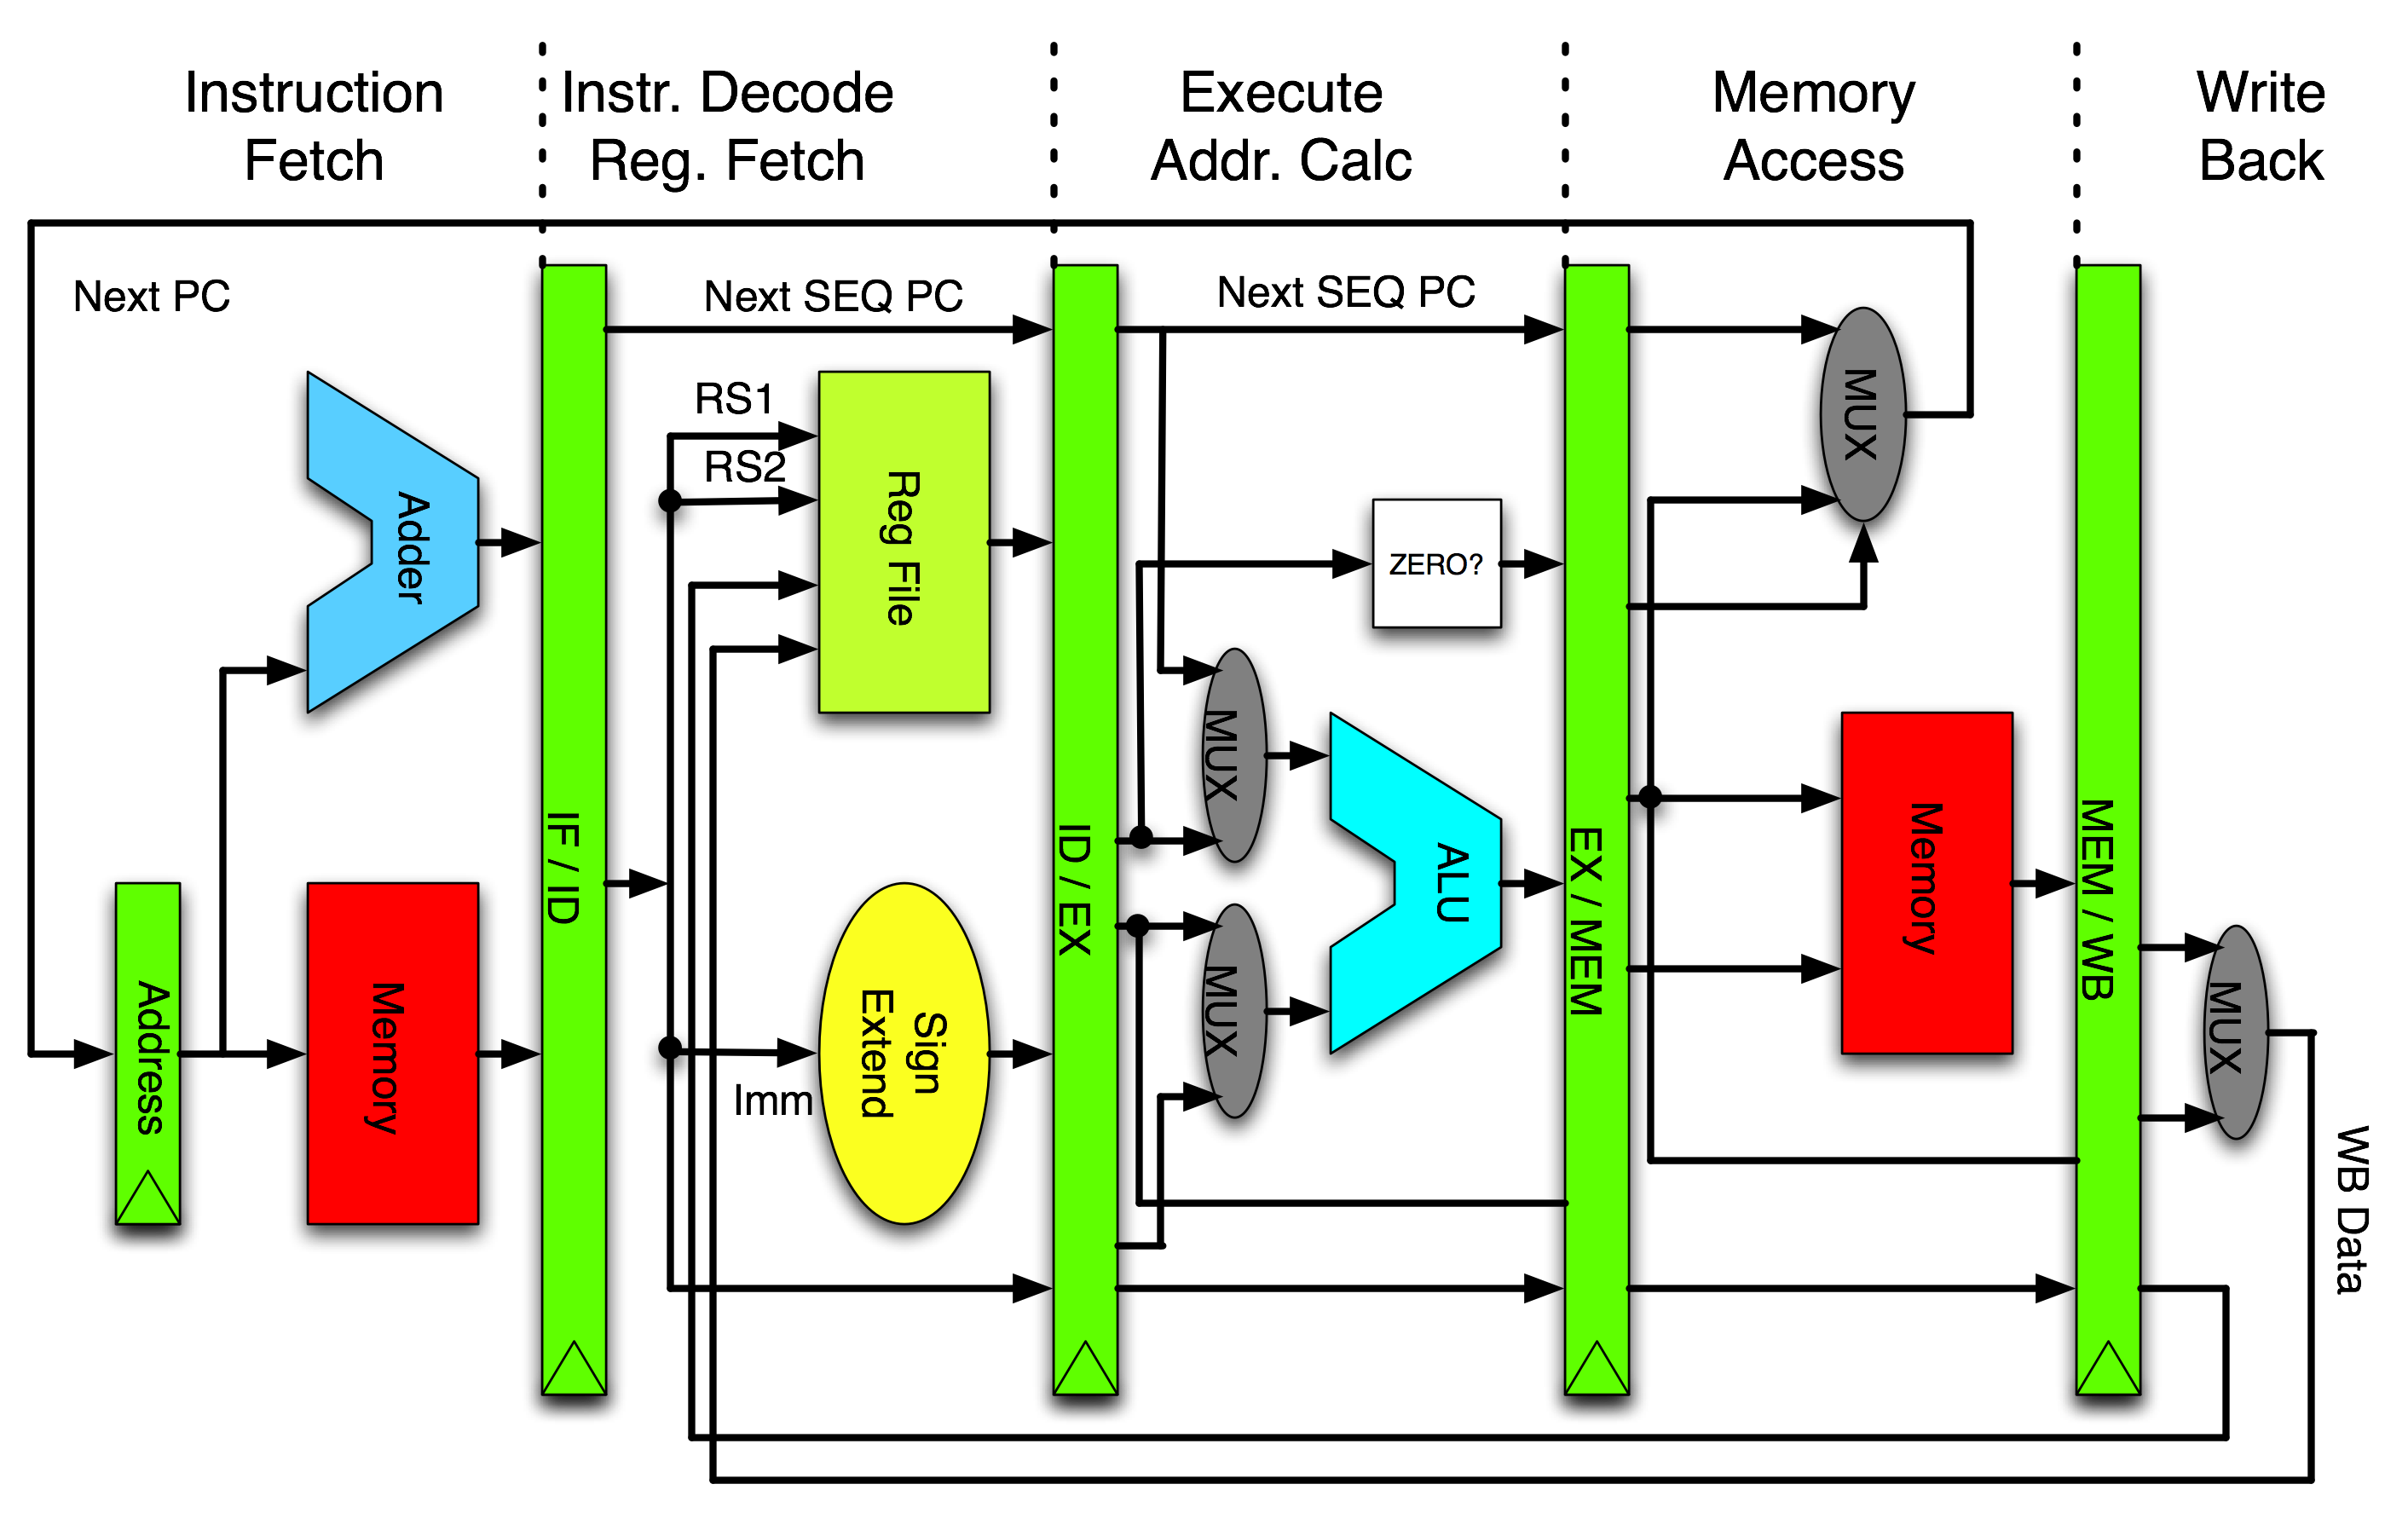
\includegraphics[width=\textwidth]{mips-pipeline.png}

  \small (MIPS, 110,000 transistors)
\end{frame}

\begin{frame}{Issues with Pipelines}
  \begin{columns}
    \column{0.5\textwidth}
      Pipelines generally help performance--but not always.

      \medskip
      Possible issue: Dependencies\dots
      \begin{itemize}
        \item \dots on memory
        \item \dots on previous computation
        \item \dots on branch outcomes
      \end{itemize}
      ``Solution'': Bubbling
    \column{0.5\textwidth}
      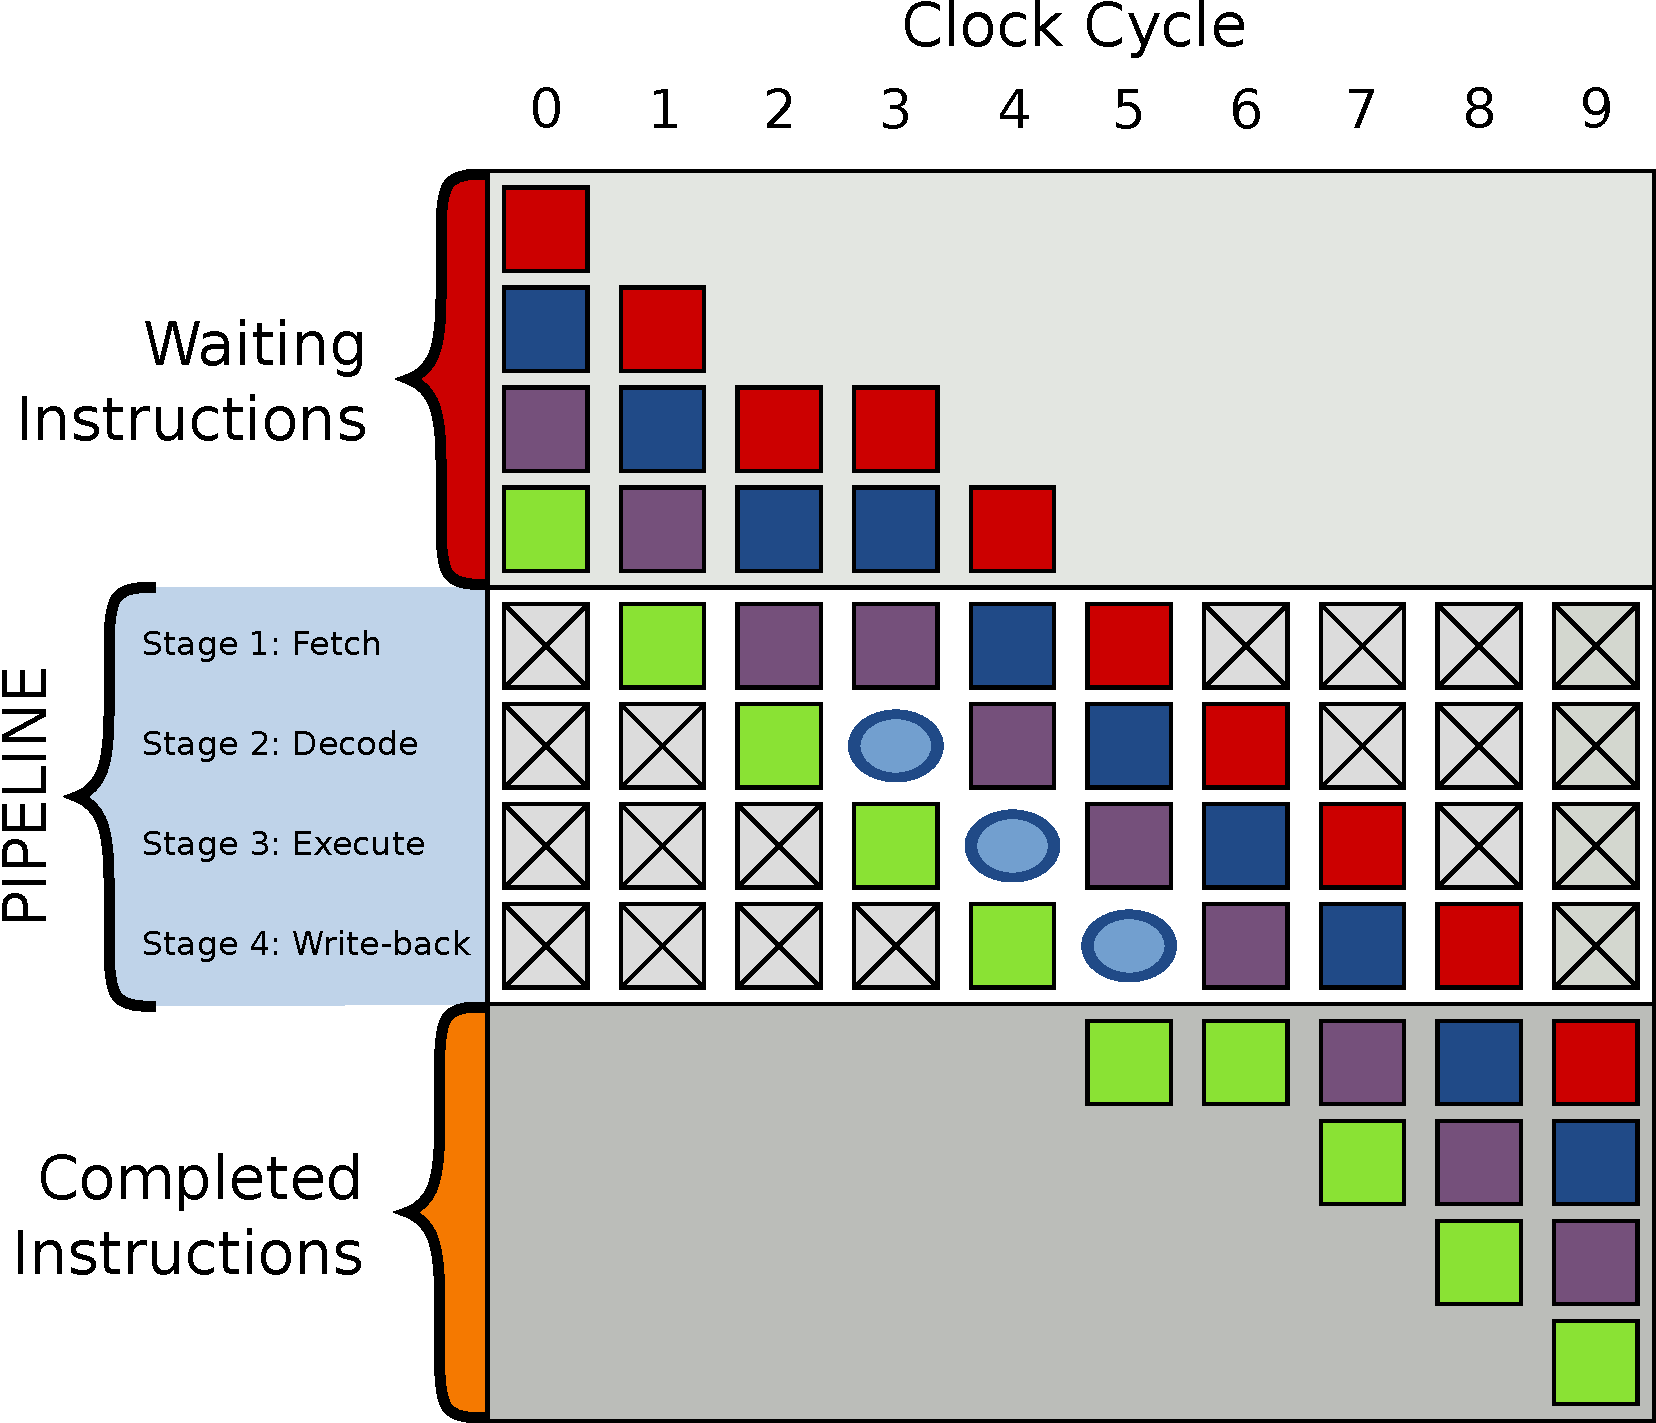
\includegraphics[width=0.8\textwidth]{pipeline-bubble.pdf}
  \end{columns}
  \uncover<2>{
    \begin{tikzpicture} [overlay]
      \node [draw,drop shadow,fill=white,anchor=south east,xshift=-0.5cm,yshift=0.5cm,
       inner sep=5mm,thick]
        at (current page.south east)
        {
          For branches: could guess\dots?
        } ;
    \end{tikzpicture}
  }
\end{frame}
\addimgcredit{Bubbly Pipeline: Wikipedia \cc}

\begin{frame}{Pipelines}
  \begin{center}
  \Huge Performance mystery demo time
  \end{center}
\end{frame}

\begin{frame}{Sandy Bridge Pipeline}
  \begin{center}
  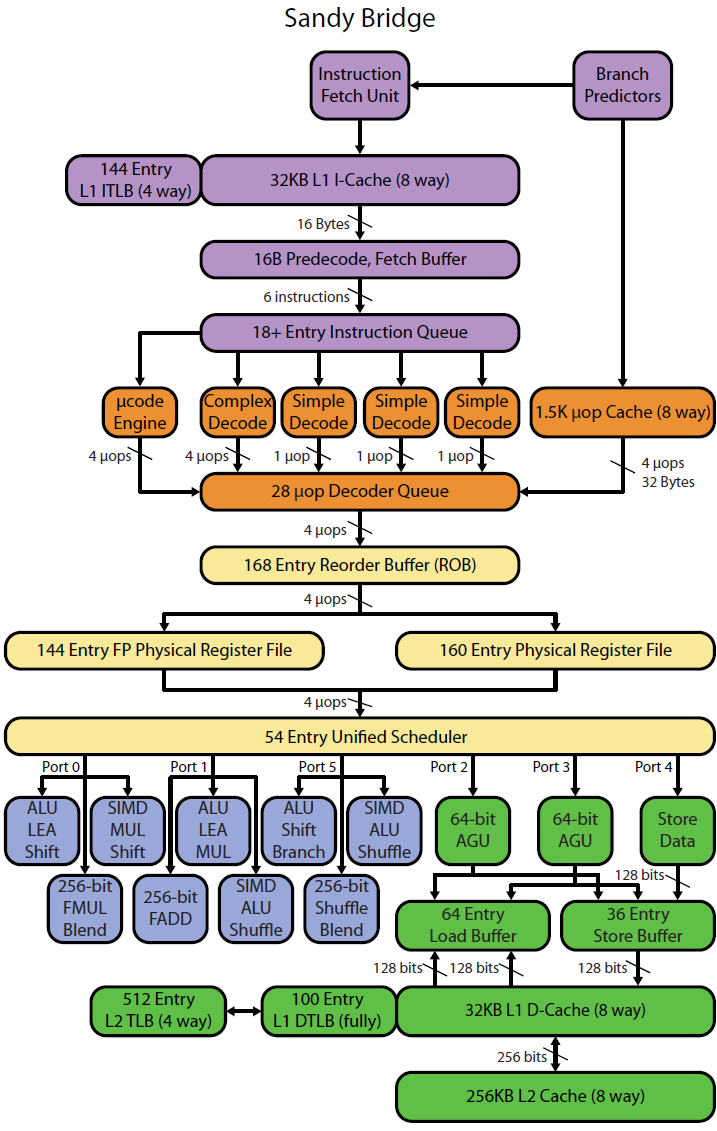
\includegraphics[height=0.85\textheight]{sandy-bridge-pipeline.png}
  \end{center}

  \creditto{David Kanter / Realworldtech.com}
  \uncover<2>{
    \begin{tikzpicture} [overlay]
      \node [draw,drop shadow,fill=white,anchor=north east,xshift=-0.5cm,yshift=-0.5cm,
      text width=0.4\textwidth, inner sep=3mm,thick]
        at (current page.north east)
        {
        New concept:\\
        Instruction-level\\
        parallelism\\
        (``Superscalar'')
        } ;
    \end{tikzpicture}
  }
\end{frame}

\begin{frame}{Programming for the Pipeline}
  How to upset a processor pipeline:
  \lstinputlisting{loop-with-if.c}

  \hfill \dots why is this bad?
\end{frame}

\begin{frame}{A Puzzle}
  \lstinputlisting{datadep.c}
  Which is faster?

  \bigskip
  \hfill \dots and why?
\end{frame}

\begin{frame}{Two useful Strategies}
  \weblink{http://en.wikipedia.org/wiki/Loop_unwinding}{Loop unrolling}:
  \begin{columns}
    \column{0.45\textwidth}
      \lstinputlisting[linerange=unr1-end]{pipeline-strategies.c}
    \column{0.05\textwidth}
      \Large$\rightarrow$
    \column{0.45\textwidth}
      \lstinputlisting[linerange=unr2-end]{pipeline-strategies.c}
  \end{columns}
  \weblink{http://en.wikipedia.org/wiki/Software_pipelining}{Software pipelining}:
  \begin{columns}
    \column{0.45\textwidth}
      \lstinputlisting[linerange=spl1-end]{pipeline-strategies.c}
    \column{0.05\textwidth}
      \Large$\rightarrow$
    \column{0.45\textwidth}
      \lstinputlisting[linerange=spl2-end]{pipeline-strategies.c}
  \end{columns}
\end{frame}
% }}}


\questionframe{}
\imagecreditslide

\end{document}
% vim: foldmethod=marker
